\section{Aerodynamic concept analysis}
\label{ch:aero_analysis}
In order to analyse the aerodynamic characteristics of the proposed concepts a software tool was developed. This chapter will deal with the development and implementation of this program. The aerodynamic tool is developed to be able to assess the performance of the different system concepts on the different trade-off criteria as defined in Chapter \ref{ch:tfsum}: the lift to drag ratio $\frac{\gls{sym:CL}}{\gls{sym:CD}}$ relates to the deceleration time and the moment stability \gls{sym:cm-alpha}\gls{sym:A} relates to the static stability of the decelerator. In order to calculate these values, the concept shapes are discretised in triangles, and for each triangle the pressure coefficient \gls{sym:cp} is calculated. This can then be integrated over the surface to obtain lift, drag and moment. The maximum heat flux $\gls{sym:qdot}_w$ is determined for each concept, which is used to determine the thermal protection system mass. 
The chapter will start with a description of the analysis method used to determine the different aerodynamic properties of the various concepts in section \ref{subsec:aerotool}. The verification and validation of the analysis tool is discussed in section \ref{subsec:aeroverval}. This will be followed by a discussion of the impact of the aerodynamic properties on the various trade-off criteria in section \ref{subsec:appaeroanal}. The chapter will conclude with the aerodynamic analysis of the various concepts in sections \ref{sec:LiftPer} to \ref{sec:AeroMom}.

\subsection{Development of aerodynamic analysis tool}
\label{subsec:aerotool}
For analysing the aerodynamic characteristics of each concept the modified Newtonian method will be used. This method relates the inclination angle $\gls{sym:chi}$ of a flat plate with respect to an incoming flow to the magnitude of its coefficient of pressure, as shown in Equation \ref{eq:modnewtonian} \cite{AndersonJr.2006}.
\begin{multicols}{2}
\begin{equation}
\gls{sym:CP}=\gls{sym:CP}_{max}sin^{2}(\gls{sym:chi})
\label{eq:modnewtonian}
\end{equation} \break
\begin{equation}
\gls{sym:CP}_{max}=\frac{p_{O_{2}}-p_{\infty}}{\frac{1}{2}\rho_{\infty}V_{\infty}^{2}}
\label{eq:cpmax}
\end{equation}
\end{multicols}
In equation \ref{eq:modnewtonian} $\gls{sym:CP}_{max}$ is the value of $\gls{sym:CP}$ in the stagnation point of an arbitrary body. Since the stagnation point is per definition located behind a normal shock its value can be found from the normal shock relations. The result of doing this is shown in Equation \ref{eq:cpmax}. Here $p_{O_{2}}$ denotes the total pressure in the stagnation point and can be found using Equation \ref{eq:po2} \cite{AndersonJr.2007}.

\begin{equation}
\frac{p_{O_{2}}}{p_{\infty}}=\left(\frac{(\gls{sym:gamma}+1)^{2}M_{\infty}^{2}}{4\gls{sym:gamma} M_{\infty}^{2}-2(\gls{sym:gamma}-1)}\right)^{\frac{\gls{sym:gamma}}{\gls{sym:gamma}-1}}\left(\frac{1-\gls{sym:gamma}+2\gls{sym:gamma} M_{\infty}^{2}}{\gls{sym:gamma}+1}\right)
\label{eq:po2}
\end{equation}

Furthermore it can be noted that $\frac{1}{2}\rho_{\infty}V_{\infty}^{2}=\frac{\gls{sym:gamma}}{2}p_{\infty}M_{\infty}^{2}$ \cite{AndersonJr.2007}. Combining this with Equation \ref{eq:cpmax} produces Equation \ref{eq:cpmaxfinal}, where the ratio $\frac{p_{O_{2}}}{p_{\infty}}$ can be calculated using Equation \ref{eq:po2}.

\begin{equation}
C_{p_{max}}=\frac{2}{\gls{sym:gamma} M_{\infty}^{2}}\left(\frac{p_{O_{2}}}{p_{\infty}}-1\right)
\label{eq:cpmaxfinal}
\end{equation}

By dividing the surface of the body to be analysed into many triangular elements the pressure coefficient distribution of said body can be determined numerically. A velocity magnitude is given as input, together with the angle of attack \gls{sym:alpha} and sideslip angle \gls{sym:beta}. Following this the outward surface normal vector is computed in Cartesian coordinates for every element, after which the velocity unit vector is computed with Equation \ref{eq:unitV}. To determine $sin(\gls{sym:chi})$ for every element the dot product of the velocity unit vector with the surface normal vector is then taken, as shown in Equation \ref{eq:dotproduct}.
\begin{multicols}{2}
\begin{equation}
\gls{sym:Vhat}=\frac{\gls{sym:Vv}}{\gls{sym:V}}
\label{eq:unitV}
\end{equation} \break
\begin{equation}
sin(\gls{sym:chi})=\gls{sym:Vhat} \bullet \gls{sym:n}
\label{eq:dotproduct}
\end{equation}
\end{multicols}
Using $C_{p_{max}}$ and $sin(\gls{sym:chi})$ the \gls{sym:CP} for every surface element is calculated, after which it is multiplied with the element area and the element surface normal vector. This results in an elemental pressure force in three dimensions from which the lift and drag forces can be determined. By then summing the resultant forces for all elements the total body forces are found. Besided the body forces, the resultant aerodynamic moment can also be found. For this the location of the \acrfull{cg} is used as input, after which the moments about the \gls{cg} caused by the force on each element can be summed. 

Two notes are made here with regard to the results produced by the Newtonian flow method:
\begin{itemize}
	\item The accuracy of the Newtonian and modified Newtonian methods increases as \gls{sym:M} become higher \cite{AndersonJr.2007,Bertin1994}
	\item Newtonian and modified Newtonian theory is more accurate for three-dimensional bodies than it is for two-dimensional cases \cite{AndersonJr.2007}
\end{itemize}

In addition to determining the aerodynamic forces and moments acting on the body, the heat flux in the stagnation point is also computed. A generalized equation to predict the heat flux on a body can be found in \cite{AndersonJr.2006,Tauber1986}. This is shown in Equation \ref{eq:heatflux}.

\begin{equation}
\gls{sym:qdot}_w=\rho_{\infty}^{N}V_{\infty}^{M}C
\label{eq:heatflux}
\end{equation}

From this same theory it is furthermore known that in the stagnation point $N=0.5$ and $M=3.0$

\begin{equation}
\label{eq:stagcoefficient}
C=1.83 \times 10^{-8} R^{-\frac{1}{2}}\left(1-\frac{h_{w}}{h_{0}}\right)
\end{equation}
Where in Equation \ref{eq:stagcoefficient} $R$ denotes the local body radius in the stagnation point and $h_{w}$ and $h_{0}$ comprise of the wall and total enthalpies respectively. An additional assumption that is made here is that $\frac{h_{w}}{h_{0}}\ll 1$. Justification for this statement can be found in the fact that the wall temperature must be smaller than the melting or decomposition temperature during the entire flight. Thus, although the temperature can become very high, the resulting wall enthalpy $h_{w}$ will still be much smaller than the total enthalpy $h_{0}$ \cite[p.347]{AndersonJr.2006}. %In addition to this the computed heat flux will increase as a result of neglecting this factor. One can see that if in later design phases the enthalpy ratio is included into the calculations this will relax the design constraints.
Combining Equations \ref{eq:heatflux} and \ref{eq:stagcoefficient} into one single Equation produces:
\begin{equation}
\gls{sym:qdot}_s=1.83 \times 10^{-8}\rho_{\infty}^{0.5} V_{\infty}^{3.0} R^{-\frac{1}{2}}
\label{eq:qstag}
\end{equation}
Where $\gls{sym:qdot}_s$ denotes the heat flux into the body at the stagnation point. This will be used as input for the thermodynamic model in order to compute the required thicknesses of the \acrfull{tps} lay-up.

\subsection{Model verification \& validation}
\label{subsec:aeroverval}
After the model construction verification was carried out to determine whether the model correctly implemented the calculations of the modified Newtonian method. This was done by placing two triangular surface elements in a flow. First at an angle and secondly normal to the flow. The model outputs were verified by also calculating the results by hand.

Following the verification process the model was validated using experimental values of different parameters. Each separate validation case will be treated here.

\subsubsection{\gls{sym:CD}-validation against experimental drag of a sphere}
\label{subsubsec:valsphere}
For the first model validation case a comparison was made the between the \gls{sym:CD}-value of a sphere in hypersonic flow that were computed by the model and as found in an experiment. It was found that for hypersonic Mach numbers the experimental \gls{sym:CD}-value of a sphere is $0.92$ \cite{Bailey1966,AndersonJr.2007,Cox1965}. When computing \gls{sym:CD} numerically with the modified Newtonian method using more than $10,000$ surface elements produces $\gls{sym:CD}=0.916$, which coincides with a discrepancy of $0.5\%$ of the experimental value. Since the accuracy of the experimental data is approximately $\pm1.5\%$ \cite{Bailey1966} this discrepancy falls within the confidence interval of the measurements.

\subsubsection{\gls{sym:CP}-validation against experimental data of a sharp cone}
\label{subsubsec:valsharpconeCP}
Following the \gls{sym:CD}-validation for blunt bodies presented in the previous section now \gls{sym:CP}-validation will be carried out for sharp bodies. This is performed by comparing \gls{sym:CP} at select points on the surface of a cone with half-cone angle \gls{sym:theta} of $15$ degrees. The experimental data was collected for $\gls{sym:M}=14.9$ and $\gls{sym:gamma}=\frac{5}{3}$  \cite{Bertin1994,Cleary1970}. Figure \ref{fig:CPcone30val} shows the data points that were collected for angles of attack $\gls{sym:alpha}=10[\deg]]$ and $\gls{sym:alpha}=20[\deg]$ in Figure \ref{fig:CPconealpha10} and \ref{fig:CPconealpha20} respectively. On the X-axis the variable \gls{sym:beta_cone} is used. This quantity refers to the local cross-sectional surface rotation with respect to an axis that is defined positive in the positive Z-direction. Figure \ref{fig:beta_cone} showcases this concept more clearly. Normally the domain of \gls{sym:beta_cone} lies between $0[\deg]$ and $360[\deg]$, but because the cone is symmetrical only half of the cone surface is plotted here. Furthermore, since the cone in question is a sharp cone with a constant semi-cone angle the \gls{sym:CP}-distribution is constant along the cone surface for constant \gls{sym:beta_cone}.
As can be seen in Figures \ref{fig:CPconealpha10} and \ref{fig:CPconealpha20} the modified Newtonian method is the most accurate around $\gls{sym:beta_cone}=90[\deg]$.

\begin{figure}[h]
	\centering
	\includegraphics[width=0.7\textwidth]{./Figure/def_beta}
	\caption{Definition of \gls{sym:beta_cone} \cite{Bertin1994}}
	\label{fig:beta_cone}
\end{figure}

\begin{figure}[h]
	\centering
	\begin{subfigure}[b]{0.49\textwidth}
		\centering
		\setlength\figureheight{0.6\textwidth} 
		\setlength\figurewidth{0.85\textwidth}
		% This file was created by matlab2tikz.
% Minimal pgfplots version: 1.3
%
\definecolor{mycolor1}{rgb}{0.20810,0.16630,0.52920}%
\definecolor{mycolor2}{rgb}{0.19855,0.72140,0.63095}%
%
\begin{tikzpicture}

\begin{axis}[%
width=0.95092\figurewidth,
height=\figureheight,
at={(0\figurewidth,0\figureheight)},
scale only axis,
xmin=0,
xmax=200,
xlabel={$\beta$ [deg]},
xmajorgrids,
ymin=0,
ymax=0.4,
ylabel={$C_p$ [-]},
ymajorgrids,
legend style={legend cell align=left,align=left,draw=white!15!black}
]
\addplot [color=mycolor1,solid]
  table[row sep=crcr]{%
0	0.313663919882391\\
4.55696202531646	0.312877849005529\\
9.11392405063291	0.310530499749308\\
13.6708860759494	0.306654244746176\\
18.2278481012658	0.301302318547099\\
22.7848101265823	0.29454775570286\\
27.3417721518987	0.286481939294681\\
31.8987341772152	0.277212794080603\\
36.4556962025316	0.266862666715091\\
41.0126582278481	0.255565942738302\\
45.5696202531646	0.243466456039843\\
50.126582278481	0.230714751131957\\
54.6835443037975	0.217465261705828\\
59.2405063291139	0.203873470516536\\
63.7974683544304	0.190093115610837\\
68.3544303797468	0.176273506281338\\
72.9113924050633	0.162557008944947\\
77.4683544303798	0.14907675848562\\
82.0253164556962	0.135954644591526\\
86.5822784810127	0.123299615408348\\
91.1392405063291	0.111206332607406\\
95.6962025316456	0.0997542029384269\\
100.253164556962	0.0890068017311918\\
104.810126582279	0.0790116938710017\\
109.367088607595	0.0698006477512688\\
113.924050632911	0.0613902278554033\\
118.481012658228	0.0537827421878944\\
123.037974683544	0.046967511998371\\
127.594936708861	0.0409224233429402\\
132.151898734177	0.0356157132021625\\
136.708860759494	0.0310079372951395\\
141.26582278481	0.0270540625330662\\
145.822784810127	0.023705624346723\\
150.379746835443	0.0209128879663695\\
154.93670886076	0.0186269531555022\\
159.493670886076	0.016801743887958\\
164.050632911392	0.0153958279571552\\
168.607594936709	0.0143740164247398\\
173.164556962025	0.0137086990254263\\
177.721518987342	0.0133808789844762\\
182.278481012658	0.0133808789844762\\
};
\addlegendentry{Modified Newtonian};

\addplot [color=mycolor2,only marks,mark=asterisk,mark options={solid}]
  table[row sep=crcr]{%
0	0.359\\
30	0.326\\
60	0.234\\
90	0.112\\
120	0.06\\
150	0.037\\
180	0.039\\
};
\addlegendentry{Measured};

\end{axis}
\end{tikzpicture}%
		\caption{$\gls{sym:alpha}=10\deg$}
		\label{fig:CPconealpha10}
	\end{subfigure}
		\begin{subfigure}[b]{0.49\textwidth}
			\centering
			\setlength\figureheight{0.6\textwidth} 
			\setlength\figurewidth{0.85\textwidth}
			% This file was created by matlab2tikz.
% Minimal pgfplots version: 1.3
%
\definecolor{mycolor1}{rgb}{0.20810,0.16630,0.52920}%
\definecolor{mycolor2}{rgb}{0.19855,0.72140,0.63095}%
%
\begin{tikzpicture}

\begin{axis}[%
width=0.95092\figurewidth,
height=\figureheight,
at={(0\figurewidth,0\figureheight)},
scale only axis,
xmin=0,
xmax=200,
xlabel={$\beta$ [deg]},
xmajorgrids,
ymin=0,
ymax=0.7,
ylabel={$C_p$ [-]},
ymajorgrids,
legend style={legend cell align=left,align=left,draw=white!15!black}
]
\addplot [color=mycolor1,solid]
  table[row sep=crcr]{%
0	0.577764228354504\\
4.55696202531646	0.575664128443356\\
9.11392405063291	0.569399969689605\\
13.6708860759494	0.559079369250394\\
18.2278481012658	0.544879022785013\\
22.7848101265823	0.527040773405377\\
27.3417721518987	0.505866243155278\\
31.8987341772152	0.481710157904938\\
36.4556962025316	0.454972528255649\\
41.0126582278481	0.426089876689746\\
45.5696202531646	0.395525724083726\\
50.126582278481	0.363760566256924\\
54.6835443037975	0.331281583018694\\
59.2405063291139	0.298572327912705\\
63.7974683544304	0.26610264639941\\
68.3544303797468	0.234319063584449\\
72.9113924050633	0.203635869964691\\
77.4683544303798	0.174427115348786\\
82.0253164556962	0.1470196975823\\
86.5822784810127	0.121687704566509\\
91.1392405063291	0.0986481360184979\\
95.6962025316456	0.0780580962897468\\
100.253164556962	0.0600135122299421\\
104.810126582279	0.044549391495899\\
109.367088607595	0.0316415978371448\\
113.924050632911	0.0212100817210665\\
118.481012658228	0.0131234681544689\\
123.037974683544	0.00720486963515046\\
127.594936708861	0.00323876168105333\\
132.151898734177	0.000978732102579191\\
136.708860759494	0.000121379574901702\\
141.26582278481	0\\
145.822784810127	0\\
150.379746835443	0\\
154.93670886076	0\\
159.493670886076	0\\
164.050632911392	0\\
168.607594936709	0\\
173.164556962025	0\\
177.721518987342	0\\
182.278481012658	0\\
};
\addlegendentry{Modified Newtonian};

\addplot [color=mycolor2,only marks,mark=asterisk,mark options={solid}]
  table[row sep=crcr]{%
0	0.63\\
30	0.55\\
60	0.327\\
90	0.093\\
120	0.028\\
150	0.009\\
180	0.014\\
};
\addlegendentry{Measured};

\end{axis}
\end{tikzpicture}%
		\caption{$\gls{sym:alpha}=20\deg$}
		\label{fig:CPconealpha20}
	\end{subfigure}
	\caption{Comparisons between experimental and numerical pressure coefficients}
	\label{fig:CPcone30val}
\end{figure}

\subsubsection{\gls{sym:CD}-validation against experimental data of a sharp cone}
\label{subsubsec:valsharpconeCD}
Stevens found that for a sharp cone-cylinder with half-cone angle \gls{sym:theta} of $30\deg$ $\gls{sym:CD}=0.58$ in an air-stream of Mach $8$ where angle of attack \gls{sym:alpha} and sideslip angle \gls{sym:beta} are zero \cite{Stevens1950,AndersonJr.2007}. The numerical model predicts for this case that $\gls{sym:CD}=0.456$, which coincides with a discrepancy of $21.4\%$ of the experimental value. This is in line with the results of section \ref{subsubsec:valsharpconeCP} where the \glspl{sym:CP} predicted by the numerical model were smaller than the experimental values of a sharp cone.

\subsubsection{\gls{sym:CP}-validation against experimental data of the Apollo re-entry capsule}
\label{subsubsec:Apollo_validation}
The data points in Figure \ref{fig:Apollo_cp} represent pressure coefficients measured at various locations of one of the two axisymmetric axes \cite{Bertin1966}. The quantity shown on the X-axis is defined in Figure \ref{fig:Apollo_y}. As can be seen in Figure \ref{fig:Apollo_cp} the numerical model is most accurate around the centre of the capsule. As the distance to the centreline increases, so does the discrepancy between the experimental and numerical values.

\begin{figure}[H]
	\centering
	\setlength\figureheight{0.4\textwidth} 
	\setlength\figurewidth{0.95\textwidth}
	% This file was created by matlab2tikz.
% Minimal pgfplots version: 1.3
%
\definecolor{mycolor1}{rgb}{0.00000,0.44700,0.74100}%
\definecolor{mycolor2}{rgb}{0.85000,0.32500,0.09800}%
%
\begin{tikzpicture}

\begin{axis}[%
width=0.95092\figurewidth,
height=\figureheight,
at={(0\figurewidth,0\figureheight)},
scale only axis,
unbounded coords=jump,
xmin=-1.5,
xmax=1.5,
xlabel={$\frac{s}{R}$ [-]},
xmajorgrids,
ymin=0,
ymax=1.8,
ylabel={$\text{C}_\text{p}\text{ [-]}$},
ymajorgrids,
legend style={at={(0.5,0.03)},anchor=south,legend cell align=left,align=left,draw=white!15!black}
]
\addplot [color=mycolor1,solid]
  table[row sep=crcr]{%
-1.095	0.00194223338446491\\
-1.09496992147514	0\\
-1.09472939221993	0.0105764109659139\\
-1.09463923908848	0\\
-1.09415883985204	0.0286612804702033\\
-1.09400885921748	0\\
-1.09328990674072	0.0560242775566994\\
-1.09308050968954	0\\
-1.09212497457122	0.092367937353207\\
-1.09185673504618	0\\
-1.09066723634165	0.137297047773714\\
-1.09034088956864	0\\
-1.08892068761116	0.190322850013229\\
-1.08853712808401	0\\
-1.08689011554844	0.250868241388263\\
-1.08645039457714	nan\\
-1.08458108581034	0.318273930108563\\
-1.0819999272869	0.3918054818373\\
-1.07915371475421	0.470661188513422\\
-1.07605024948299	0.55398068095838\\
-1.07269803785581	0.640854198362098\\
-1.06910626805175	0.730332419944821\\
-1.06528478486218	0.821436757031353\\
-1.06124406270688	0.913169997566455\\
-1.05699517692443	1.00452718986455\\
-1.05254977341541	1.09450664823589\\
-1.04792003672184	1.18212096017887\\
-1.0431186566302	1.26640787317747\\
-1.03815879338958	1.34644093888065\\
-1.03305404164036	1.42133979364298\\
-1.02781839315226	1.42835417521564\\
-1.01832656548985	1.44935521736688\\
-0.986104624404206	1.50751538767456\\
-0.953709183690762	1.52351962805163\\
-0.921145943147255	1.5390688207566\\
-0.888420632094868	1.55415195599687\\
-0.855539008370191	1.56875835245074\\
-0.822506857312158	1.58287766497233\\
-0.789329990744154	1.59649989205813\\
-0.75601424595145	1.60961538306931\\
-0.72256548465417	1.62221484520418\\
-0.688989591975953	1.63428935021542\\
-0.655292475408497	1.64583034086682\\
-0.621480063772172	1.6568296371244\\
-0.587558306172872	1.66727944207735\\
-0.553533170955306	1.67717234758383\\
-0.519410644652901	1.68650133963741\\
-0.485196730934503	1.69525980344988\\
-0.450897449548067	1.7034415282464\\
-0.416518835261513	1.71104071176934\\
-0.382066936800948	1.71805196448708\\
-0.347547815786417	1.72447031350459\\
-0.312967545665402	1.7302912061727\\
-0.27833221064423	1.73551051339311\\
-0.243647904617593	1.74012453261658\\
-0.208920730096357	1.74412999053202\\
-0.174156797133862	1.74752404544416\\
-0.139362222250891	1.7503042893381\\
-0.104543127359504	1.75246874962895\\
-0.0697056386859186	1.75401589059533\\
-0.0348558856926369	1.75488268492153\\
-0	1.75525426236477\\
0.0348558856926369	1.75488268492153\\
0.0697056386859186	1.75401589059533\\
0.104543127359504	1.75246874962895\\
0.139362222250891	1.7503042893381\\
0.174156797133862	1.74752404544416\\
0.208920730096357	1.74412999053202\\
0.243647904617593	1.74012453261658\\
0.27833221064423	1.73551051339311\\
0.312967545665402	1.7302912061727\\
0.347547815786417	1.72447031350459\\
0.382066936800948	1.71805196448708\\
0.416518835261513	1.71104071176934\\
0.450897449548067	1.7034415282464\\
0.485196730934503	1.69525980344988\\
0.519410644652901	1.68650133963741\\
0.553533170955306	1.67717234758383\\
0.587558306172872	1.66727944207735\\
0.621480063772172	1.6568296371244\\
0.655292475408497	1.64583034086682\\
0.688989591975953	1.63428935021542\\
0.72256548465417	1.62221484520418\\
0.75601424595145	1.60961538306931\\
0.789329990744154	1.59649989205813\\
0.822506857312158	1.58287766497233\\
0.855539008370191	1.56875835245074\\
0.888420632094868	1.55415195599687\\
0.921145943147255	1.5390688207566\\
0.953709183690762	1.52351962805163\\
0.986104624404206	1.50751538767456\\
1.01832656548985	1.44935521736688\\
1.02781839315226	1.42835417521564\\
1.03305404164036	1.42133979364298\\
1.03815879338958	1.34644093888065\\
1.0431186566302	1.26640787317747\\
1.04792003672184	1.18212096017886\\
1.05254977341541	1.09450664823589\\
1.05699517692443	1.00452718986455\\
1.06124406270688	0.913169997566455\\
1.06528478486218	0.821436757031353\\
1.06910626805175	0.730332419944821\\
1.07269803785581	0.640854198362098\\
1.07605024948299	0.55398068095838\\
1.07915371475421	0.470661188513422\\
1.0819999272869	0.3918054818373\\
1.08458108581034	0.318273930108563\\
1.08645039457714	nan\\
1.08689011554844	0.250868241388263\\
1.08853712808401	0\\
1.08892068761116	0.190322850013229\\
1.09034088956864	0\\
1.09066723634165	0.137297047773714\\
1.09185673504618	0\\
1.09212497457122	0.0923679373532069\\
1.09308050968954	0\\
1.09328990674072	0.0560242775566994\\
1.09400885921748	0\\
1.09415883985204	0.0286612804702033\\
1.09463923908848	0\\
1.09472939221993	0.0105764109659139\\
1.09496992147514	0\\
1.095	0.0019422333844649\\
};
\addlegendentry{Modified Newtonian};

\addplot [color=mycolor2,only marks,mark=asterisk,mark options={solid}]
  table[row sep=crcr]{%
-1.02718093698553	0.326751322056051\\
-0.951551131339198	1.02168543257076\\
-0.799264139197169	1.4880212545932\\
-0.247616441864002	1.7300201625693\\
0.0180691662280614	1.74873159897289\\
0.273850147488554	1.70299372722051\\
0.547682381293604	1.63105638244619\\
0.68183629061674	1.49350323432687\\
0.817930550476365	1.44043342939967\\
0.871460439771112	1.37207156639853\\
0.929404854806911	1.26182928317321\\
0.981710021888355	0.939565894363321\\
1.0408671541418	0.31807000221393\\
1.09530512997895	0.0391870122023066\\
};
\addlegendentry{Measured};

\end{axis}
\end{tikzpicture}%
	\caption{Comparison between experimental and numerical \glspl{sym:CP} for the Apollo re-entry capsule}
	\label{fig:Apollo_cp}
\end{figure}

\begin{figure}[H]
	\centering
	\includegraphics[width=0.4\textwidth]{./Figure/Apollo_model}
	\caption{Definition of unit on the horizontal axis of Figure \ref{fig:Apollo_cp} \cite{Bertin1966}}
	\label{fig:Apollo_y}
\end{figure}

\subsubsection{Maximum heat flux validation against experimental data of the \gls{irve} 3 vehicle}
\label{subsubsec:heatvalidation}
Dillman et al. observed that the maximum heat flux on the \acrfull{irve} 3 was $14.4$ $\frac{W}{cm^{2}}$ during re-entry at an altitude of $50$ kilometres and Mach $7.0$ \cite{Dillman2012}. The maximum heat flux computed by the numerical tool in the stagnation point for these flow conditions is $11.7$ $\frac{W}{cm^{2}}$. This is equal to $81.0\%$ of the experimental value. Thus a discrepancy of $19.0\%$ is present between the experimental and numerical maximum heat fluxes.

\subsubsection{Conclusions after the validation procedure}
\label{subsec:validconclusions}
From section \ref{subsec:aeroverval} it can be seen that the accuracy of the modified Newtonian method varies between geometries. The \gls{sym:CD} predicted in section \ref{subsubsec:valsphere} is accurate to within $1\%$ of the experimental value, whereas the accuracy of the \glspl{sym:CP} in section \ref{subsubsec:valsharpconeCP} varied over the cone surface. This discrepancy was also seen in section \ref{subsubsec:valsharpconeCD}, where the difference between the numerical and experimental \gls{sym:CD} was $21.4\%$, and again for the Apollo capsule in section \ref{subsubsec:Apollo_validation}. After judging the accuracy shown in Figures \ref{fig:CPcone30val} and \ref{fig:Apollo_cp} it was determined that the accuracy of the modified Newtonian method is adequate for the conceptual and preliminary design phases.
The model for the maximum heat flux found on a body was validated in section \ref{subsubsec:heatvalidation}. It was observed that a discrepancy of $19.0\%$ was present between the numerical and experimental maximum heat fluxes. After consideration this was deemed to be acceptable for conceptual and preliminary design.

\subsection{Application of analysis tool to system concepts}
\label{subsec:appaeroanal}
After the model development and validation, the different system concepts are evaluated on performance in the different trade-off criteria. Specifically, the lift, moment and aerodynamic heating are discussed. They are all related to the trade-off criteria as defined in Chapter \ref{ch:tradeoff}. Firstly, the relation between the aerodynamic properties and the trade-off criteria is discussed. After that, the results from the aerodynamic analysis is given.



\subsubsection{Trade-off criteria justification} \label{sec:tradeoffaero}
In this section, the quantification method of the trade-off criteria relating to aerodynamics is justified.

The stability trade-off criterion is given by the static stability of the vehicle. This is characterised by the pitch moment gradient \gls{sym:cm-alpha}\gls{sym:A}: For a negative \gls{sym:cm-alpha}\gls{sym:A}, a positive angle of attack leads to a negative moment, such that the angle of attack is restored by the induced moment. This leads to a spacecraft that is less reactant to disturbances in the atmosphere, which leads to a less strict requirement on the control system to keep the spacecraft pointed in the desired direction. A positive value of \gls{sym:cm-alpha}\gls{sym:A} means the spacecraft is not stable, and the control system will have to constantly monitor and control the spacecraft in order for it to not diverge from the required attitude. \\


Aerodynamic drag is used as the method to decelerate the vehicle from the initial velocity to $\gls{sym:M}=5$ before landing. The drag equation is given in Eq. \ref{eq:drag}.

\begin{equation} \label{eq:drag}
\gls{sym:D} = \frac{1}{2}\gls{sym:rho}\gls{sym:V}^2\gls{sym:CD}\gls{sym:A}
\end{equation}
\begin{equation} \label{eq:lift}
\gls{sym:L} = \frac{1}{2}\gls{sym:rho}\gls{sym:V}^2\gls{sym:CL}\gls{sym:A}
\end{equation}

The lift is defined as the component of the aerodynamic force perpendicular to the flow, where the direction away from Mars is defined positive. The drag component is defined parallel to the flow. For blunt bodies in hypersonic flow with the blunt side pointed towards the oncoming flow, a positive angle of attack results in a negative lift.

The drag and lift are dependent on the drag and lift coefficients of the spacecraft as well as the density. As can be seen in Figure \ref{fig:atmos_height_rho}, the density is significantly higher in lower parts of the atmosphere. For a given \gls{sym:CD}\gls{sym:A}, the maximum deceleration can be chosen by varying the lowest part of the orbit: a higher density compensates for a low drag coefficient to produce the same force as a spacecraft with a high drag coefficient and a low density. Because of the large variation of density in the atmosphere, it is possible to find a trajectory for any \gls{sym:CD}\gls{sym:A}. Thus, the drag coefficient itself is not a key driver for the design. However, the spacecraft can influence its deceleration time in the atmosphere by producing lift: if the spacecraft were to fly out of the atmosphere, a downward pointing lift would divert it's trajectory more through the atmosphere. The ability of the spacecraft to influence this trajectory through the atmosphere is characterised by the amount of lift that can be produced, with respect to the amount of drag produced at the same \gls{sym:alpha}. The dependence on drag is due to the fact that two spacecraft with the same $\frac{\gls{sym:CL}}{\gls{sym:CD}}$ but a different \gls{sym:CD}\gls{sym:A}, will just have the lowest part of the trajectory in a different height, where the total lift and drag force will be the same for both spacecraft. Therefore, the deceleration time is characterised by $\frac{\gls{sym:CL}}{\gls{sym:CD}}$. \\

The mass of the decelerator is composed of the structural mass, the \gls{tps} mass and the control system mass. 
The \gls{tps} mass is estimated based on the heat load on the spacecraft, which is the integral of the heat flux over time. This heat load is the total amount of heat supplied to the spacecraft between initial entry and final descent, and estimates the total amount of energy the \gls{tps} has to withstand. This can thus be used to size the thickness of the \gls{tps}, which leads directly to the mass of the system.
The control system mass is based on the moment that the control system has to provide. The spacecraft has to fly at a given lift to drag ratio to maintain its trajectory. These lift to drag ratios are obtained at a certain angle of attack. This angle of attack in turn corresponds to a moment produced by the spacecraft. To maintain a stable trajectory, this moment needs to be counteracted by the spacecraft control systems. The greater the moment that needs to be counteracted, the greater the required control system mass will be. Therefore the ratio between the lift to drag ratio required and the moment coefficient that is required to maintain this lift to drag ratio will indicate the required control system mass. This ratio is given by $\frac{\gls{sym:CM}}{\gls{sym:CL}/\gls{sym:CD}}$.

In order to assess these values, a representative geometry is chosen. Since Newtonian flow only affects the parts of the vehicle that are in direct line of sight of the oncoming flow, only the front of the decelerator has to be accurately modelled. The stacked toroid and tension cone concepts are modelled after the \gls{irve} missions as flown by NASA, as can be seen in Figure \ref{fig:cpstackedtoroid}. The isotensoid model is modelled as a slightly flattened sphere, with a radius of 6 meters perpendicular and a radius of 5 meter in direction of the flow. This model can be seen in Figure \ref{fig:cpisotensoid}. The Trailing ballute is modelled as a single torus trailing body comparable to the rigid concept., as seen in Figure \ref{fig:cpballute}, and the rigid concept's front is a largely flattened sphere, as seen in Figure \ref{fig:cprigid}.


\begin{figure}[h]
	\centering
	\begin{subfigure}[b]{0.49\textwidth}
		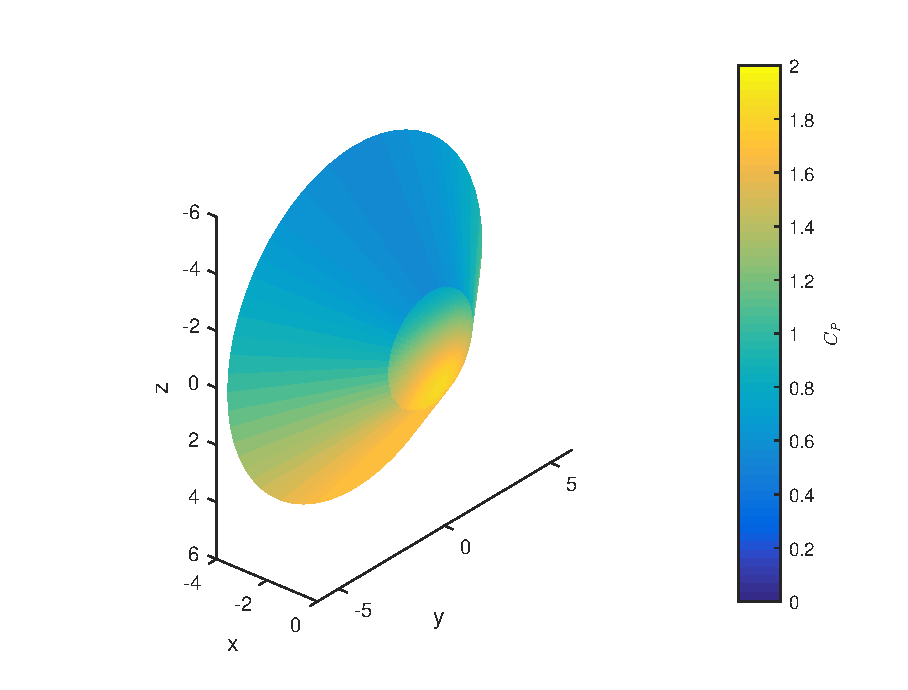
\includegraphics[width=0.96\textwidth]{./Figure/aero_model/irve.eps}
		\caption{Stacked toroid, tension cone}
		\label{fig:cpstackedtoroid}
	\end{subfigure}
	\begin{subfigure}[b]{0.49\textwidth}
		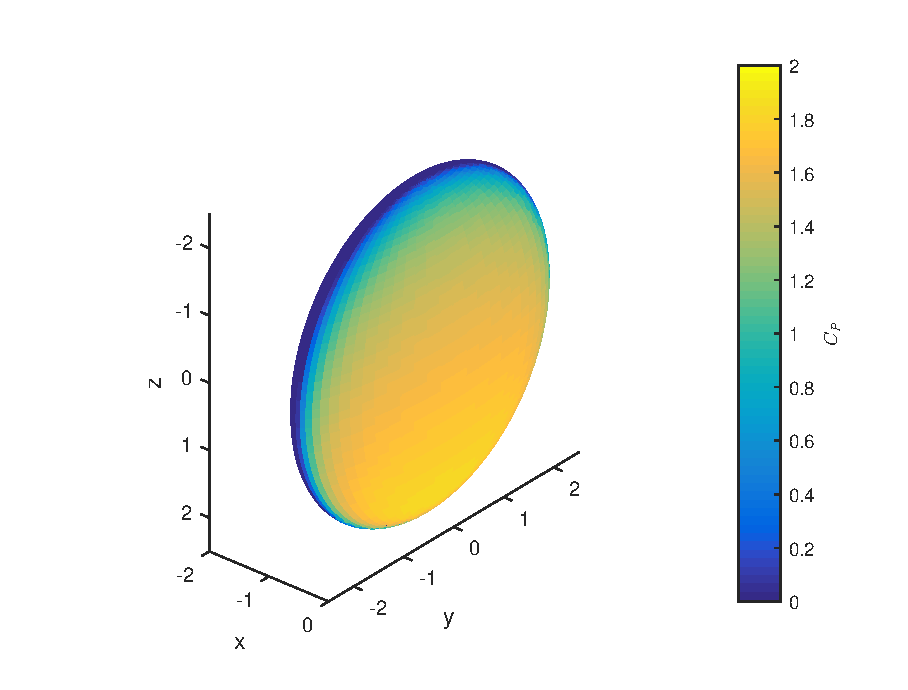
\includegraphics[width=0.96\textwidth]{./Figure/aero_model/rigid.eps}
		\caption{Rigid structure}
		\label{fig:cprigid}
	\end{subfigure}
	\begin{subfigure}[b]{0.49\textwidth}
		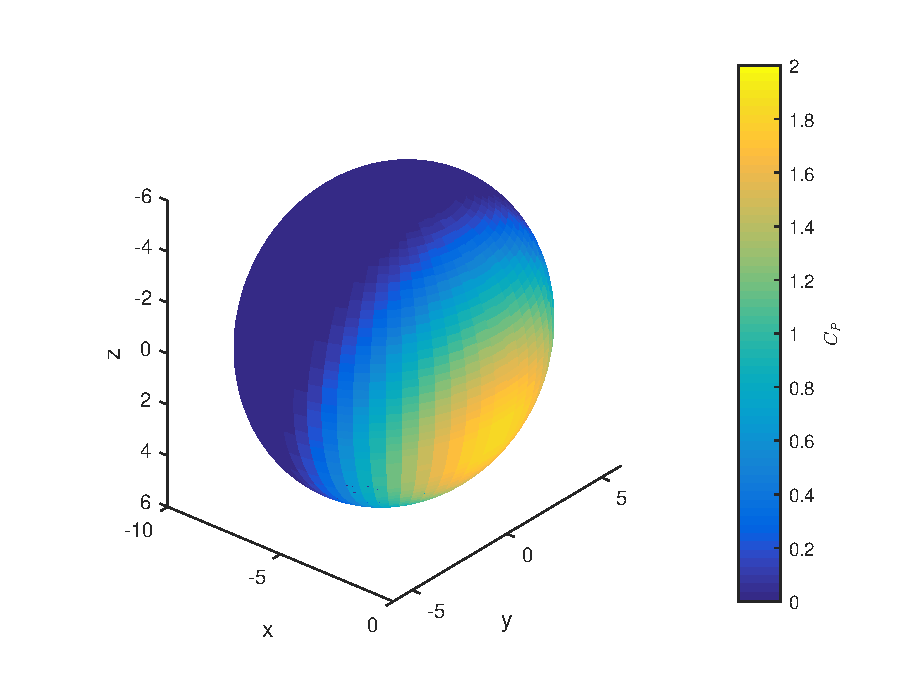
\includegraphics[width=0.96\textwidth]{./Figure/aero_model/isotensoid.eps}
		\caption{Isotensoid}
		\label{fig:cpisotensoid}
	\end{subfigure}
	\begin{subfigure}[b]{0.49\textwidth}
		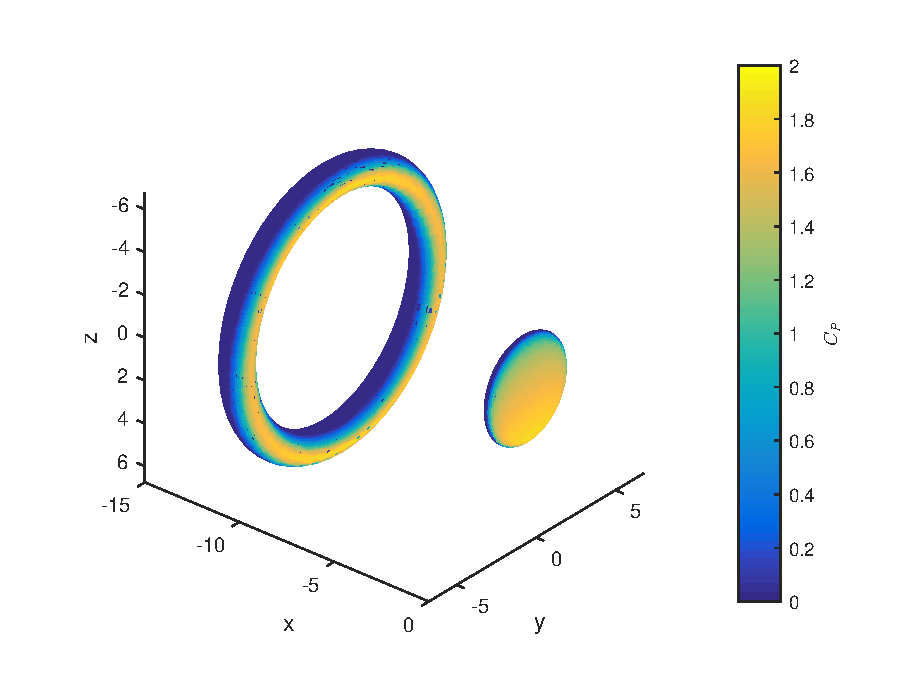
\includegraphics[width=0.96\textwidth]{./Figure/aero_model/ballute.eps}
		\caption{Trailing ballute}
		\label{fig:cpballute}
	\end{subfigure}	
	\caption{Geometry and pressure coefficient \gls{sym:CP} distribution over the different concepts, at an angle of attack $\gls{sym:alpha}=20[deg]$. }
	\label{fig:conceptscp}
\end{figure}

\subsubsection{Lift performance}
\label{sec:LiftPer}
The lift is defined as the component of the aerodynamic force perpendicular to the flow, where the direction away from Mars is defined positive. The Equation used to calculate the total lift of a vehicle is given in Eq \ref{eq:lift}.
\begin{equation}
\gls{sym:L} = \frac{1}{2}\gls{sym:rho}\gls{sym:V}^2\gls{sym:CL}\gls{sym:A}
\label{eq:lift}
\end{equation}
This $\gls{sym:CL}\gls{sym:A}$ is the lift coefficient multiplied with the reference area and as such gives insight in the lift generation of a given spacecraft, incorporating its size. For blunt vehicles with a blunt surface perpendicular to the flow, a positive angle of attack $\gls{sym:alpha}$ results in a negative lift.

In Figure \ref{fig:clplots}, the lift coefficient can be seen to vary greatly for the different concepts: the stacked toroid and tension cone produce about 3 times the lift of the other concepts. This is also reflected in the lift gradient plot, which can be found in \ref{fig:claplha}. The lift gradient plot is the graph that provides the information needed for the trade-off, since the lift gradient determines how much the control system has to change the angle of attack to achieve a given lift. It is clear that the stacked toroid and tension cone have the greatest lift and lift gradient, while the trailing ballute follows closely. The other two concepts offer a significantly less lift performance. The lift to drag ratios of the various concepts at an angle of attack of $\gls{sym:alpha}=20^\circ$ are summarized in Table \ref{tab:clcd}.



\subsubsection{Deceleration performance}
$\frac{\gls{sym:CL}}{\gls{sym:CD}}$ is the lift coefficient divided by the drag coefficient. In Figure \ref{fig:clcd}, a graph is presented showing the lift over drag ratios of the different concepts for different angles of attack.


\begin{figure}[h]
	\centering
	\begin{subfigure}{0.49\textwidth}
		\setlength\figureheight{0.8\textwidth} 
		\setlength\figurewidth{0.75\textwidth}
		% This file was created by matlab2tikz.
% Minimal pgfplots version: 1.3
%
\definecolor{mycolor1}{rgb}{0.00000,0.44700,0.74100}%
\definecolor{mycolor2}{rgb}{0.85000,0.32500,0.09800}%
\definecolor{mycolor3}{rgb}{0.92900,0.69400,0.12500}%
\definecolor{mycolor4}{rgb}{0.49400,0.18400,0.55600}%
%
\begin{tikzpicture}

\begin{axis}[%
width=\figurewidth,
height=0.802158\figureheight,
at={(0\figurewidth,0\figureheight)},
scale only axis,
xmin=0,
xmax=60,
xlabel={$\alpha [deg]$},
xmajorgrids,
ymin=-1.2,
ymax=0.2,
ylabel={$\frac{C_L}{C_D} [-]$},
ymajorgrids,
axis x line*=bottom,
axis y line*=left,
legend style={at={(0.5,1.03)},anchor=south,legend cell align=left,align=left,draw=white!15!black}
]
\addplot [color=mycolor1,solid]
  table[row sep=crcr]{%
0	5.0364332293734e-17\\
1.01694915254237	-0.00886881038686472\\
2.03389830508475	-0.0177382765063238\\
3.05084745762712	-0.0266105083780653\\
4.06779661016949	-0.0354886933600949\\
5.08474576271186	-0.0443715105173429\\
6.10169491525424	-0.0532604572812532\\
7.11864406779661	-0.0621615184206523\\
8.13559322033898	-0.0710632131161607\\
9.15254237288135	-0.0799833143202747\\
10.1694915254237	-0.0889186009161462\\
11.1864406779661	-0.0978673650802531\\
12.2033898305085	-0.106836247271851\\
13.2203389830508	-0.115822465346637\\
14.2372881355932	-0.124823767028197\\
15.2542372881356	-0.13385762066535\\
16.271186440678	-0.14291508431104\\
17.2881355932203	-0.151998683525364\\
18.3050847457627	-0.161112597537135\\
19.3220338983051	-0.170258068271788\\
20.3389830508475	-0.179437846131841\\
21.3559322033898	-0.18866733028304\\
22.3728813559322	-0.197935572390311\\
23.3898305084746	-0.207246231336731\\
24.4067796610169	-0.216610676843288\\
25.4237288135593	-0.226029079788545\\
26.4406779661017	-0.235500402027576\\
27.4576271186441	-0.245048797158496\\
28.4745762711864	-0.254675524395709\\
29.4915254237288	-0.264368970690935\\
30.5084745762712	-0.274144565505753\\
31.5254237288136	-0.284000869710777\\
32.5423728813559	-0.293963000520449\\
33.5593220338983	-0.304046514060793\\
34.5762711864407	-0.314230454783092\\
35.593220338983	-0.324548428710094\\
36.6101694915254	-0.334995581514627\\
37.6271186440678	-0.345581250359487\\
38.6440677966102	-0.356350505539155\\
39.6610169491525	-0.367299029893162\\
40.6779661016949	-0.378437450608654\\
41.6949152542373	-0.389774409373945\\
42.7118644067797	-0.401343527185476\\
43.728813559322	-0.41316823288265\\
44.7457627118644	-0.425261011495103\\
45.7627118644068	-0.437653761709246\\
46.7796610169491	-0.450372618961619\\
47.7966101694915	-0.463449434162733\\
48.8135593220339	-0.476919208845705\\
49.8305084745763	-0.49082191311632\\
50.8474576271186	-0.505195519628189\\
51.864406779661	-0.52009645855347\\
52.8813559322034	-0.53556657562102\\
53.8983050847458	-0.551648196470665\\
54.9152542372881	-0.568283757276648\\
55.9322033898305	-0.585449875597817\\
56.9491525423729	-0.603102595782494\\
57.9661016949153	-0.621254764307888\\
58.9830508474576	-0.63997775013727\\
60	-0.659105608112932\\
};
\addlegendentry{Stacked Toroid, Tension Cone};

\addplot [color=mycolor2,solid]
  table[row sep=crcr]{%
0	-1.483383500215e-17\\
1.01694915254237	-0.0154466075973433\\
2.03389830508475	-0.0308983215205245\\
3.05084745762712	-0.0463610560478669\\
4.06779661016949	-0.0618446102232318\\
5.08474576271186	-0.0773505143140998\\
6.10169491525424	-0.0928846627742007\\
7.11864406779661	-0.108456004644763\\
8.13559322033898	-0.124060991440119\\
9.15254237288135	-0.139718543875477\\
10.1694915254237	-0.155430602443469\\
11.1864406779661	-0.171192864752111\\
12.2033898305085	-0.187025937831282\\
13.2203389830508	-0.202926542000502\\
14.2372881355932	-0.218894684168724\\
15.2542372881356	-0.234955117035483\\
16.271186440678	-0.251097330959081\\
17.2881355932203	-0.267325606621165\\
18.3050847457627	-0.283660857944599\\
19.3220338983051	-0.300097464002817\\
20.3389830508475	-0.316642583385728\\
21.3559322033898	-0.333303073436136\\
22.3728813559322	-0.350089018916926\\
23.3898305084746	-0.366999519799466\\
24.4067796610169	-0.384038482704838\\
25.4237288135593	-0.401209914092416\\
26.4406779661017	-0.418523695535869\\
27.4576271186441	-0.435985520643127\\
28.4745762711864	-0.45360606313891\\
29.4915254237288	-0.471391353616969\\
30.5084745762712	-0.4893223886892\\
31.5254237288136	-0.507417402286324\\
32.5423728813559	-0.525683568328429\\
33.5593220338983	-0.544103614941209\\
34.5762711864407	-0.56271670835948\\
35.593220338983	-0.581467260500827\\
36.6101694915254	-0.600388686064697\\
37.6271186440678	-0.619538178488193\\
38.6440677966102	-0.638815202222698\\
39.6610169491525	-0.65824500237328\\
40.6779661016949	-0.677841541292329\\
41.6949152542373	-0.697594877563252\\
42.7118644067797	-0.717460352349361\\
43.728813559322	-0.737481568527868\\
44.7457627118644	-0.757558996246075\\
45.7627118644068	-0.777789489185058\\
46.7796610169491	-0.798056114960774\\
47.7966101694915	-0.818317974641001\\
48.8135593220339	-0.838694944944911\\
49.8305084745763	-0.858950873214175\\
50.8474576271186	-0.879168337136622\\
51.864406779661	-0.899186236656746\\
52.8813559322034	-0.919089659008339\\
53.8983050847458	-0.938685318744582\\
54.9152542372881	-0.957937250327412\\
55.9322033898305	-0.976734437860176\\
56.9491525423729	-0.99497687539228\\
57.9661016949153	-1.01253569606119\\
58.9830508474576	-1.02934147729458\\
60	-1.04504382349516\\
};
\addlegendentry{Rigid};

\addplot [color=mycolor3,solid]
  table[row sep=crcr]{%
0	-1.90537580047186e-17\\
1.01694915254237	-0.00388449332173622\\
2.03389830508475	-0.0077711352640538\\
3.05084745762712	-0.0116588219579171\\
4.06779661016949	-0.0155409246522078\\
5.08474576271186	-0.0194088377935679\\
6.10169491525424	-0.0232625567357673\\
7.11864406779661	-0.0270974626647968\\
8.13559322033898	-0.0309045560337592\\
9.15254237288135	-0.0346868341158774\\
10.1694915254237	-0.0384345188395192\\
11.1864406779661	-0.0421445747251795\\
12.2033898305085	-0.0458169197904375\\
13.2203389830508	-0.0494502569125963\\
14.2372881355932	-0.0530371084378388\\
15.2542372881356	-0.056576648472266\\
16.271186440678	-0.0600592684285724\\
17.2881355932203	-0.0634864072750192\\
18.3050847457627	-0.0668559233344702\\
19.3220338983051	-0.0701641858629192\\
20.3389830508475	-0.0734106705211148\\
21.3559322033898	-0.0765839440703246\\
22.3728813559322	-0.0796808825502233\\
23.3898305084746	-0.0826986669147268\\
24.4067796610169	-0.0856394063459\\
25.4237288135593	-0.0884977329936396\\
26.4406779661017	-0.0912686931180848\\
27.4576271186441	-0.0939468736822213\\
28.4745762711864	-0.0965291977703355\\
29.4915254237288	-0.0990099320252114\\
30.5084745762712	-0.101393982347161\\
31.5254237288136	-0.103669318481619\\
32.5423728813559	-0.105841249157396\\
33.5593220338983	-0.107901939900376\\
34.5762711864407	-0.109841974772035\\
35.593220338983	-0.111651588839047\\
36.6101694915254	-0.113351717263537\\
37.6271186440678	-0.114927213048414\\
38.6440677966102	-0.11637293487655\\
39.6610169491525	-0.117677581483272\\
40.6779661016949	-0.118840943288529\\
41.6949152542373	-0.119880718640198\\
42.7118644067797	-0.120780216790739\\
43.728813559322	-0.121526977373284\\
44.7457627118644	-0.122123248053378\\
45.7627118644068	-0.122570601134165\\
46.7796610169491	-0.122871597151468\\
47.7966101694915	-0.123024818608255\\
48.8135593220339	-0.123010783232722\\
49.8305084745763	-0.122835509599402\\
50.8474576271186	-0.122501611583236\\
51.864406779661	-0.122011984834728\\
52.8813559322034	-0.121364823591745\\
53.8983050847458	-0.120548104510166\\
54.9152542372881	-0.119565153864216\\
55.9322033898305	-0.118403165245806\\
56.9491525423729	-0.117098457136955\\
57.9661016949153	-0.115630804835734\\
58.9830508474576	-0.113978607232654\\
60	-0.112175112033318\\
};
\addlegendentry{Isotensoid};

\addplot [color=mycolor4,solid]
  table[row sep=crcr]{%
0	-2.28022995225568e-17\\
1.01694915254237	-0.0109039532707526\\
2.03389830508475	-0.0218103459567605\\
3.05084745762712	-0.0327169986285077\\
4.06779661016949	-0.0436329837997838\\
5.08474576271186	-0.0545464969621898\\
6.10169491525424	-0.0654591033129618\\
7.11864406779661	-0.0763408429945217\\
8.13559322033898	-0.087179804352967\\
9.15254237288135	-0.0979914069080698\\
10.1694915254237	-0.108764158113581\\
11.1864406779661	-0.119498605569514\\
12.2033898305085	-0.130189386360552\\
13.2203389830508	-0.140848593828011\\
14.2372881355932	-0.151465879586014\\
15.2542372881356	-0.162041030492625\\
16.271186440678	-0.172558252582399\\
17.2881355932203	-0.183004895775267\\
18.3050847457627	-0.193378433979145\\
19.3220338983051	-0.203664649485995\\
20.3389830508475	-0.213851966443941\\
21.3559322033898	-0.223944370362439\\
22.3728813559322	-0.233935361308867\\
23.3898305084746	-0.243813793907642\\
24.4067796610169	-0.253579681430793\\
25.4237288135593	-0.263221820330201\\
26.4406779661017	-0.272722180985976\\
27.4576271186441	-0.282064785017106\\
28.4745762711864	-0.291231570106086\\
29.4915254237288	-0.300203697633695\\
30.5084745762712	-0.308977133971422\\
31.5254237288136	-0.317531899314625\\
32.5423728813559	-0.325854578170721\\
33.5593220338983	-0.333945089423567\\
34.5762711864407	-0.341779350568318\\
35.593220338983	-0.349334267939829\\
36.6101694915254	-0.356587058328937\\
37.6271186440678	-0.363513901990876\\
38.6440677966102	-0.370082642652605\\
39.6610169491525	-0.376273577369382\\
40.6779661016949	-0.382060152503511\\
41.6949152542373	-0.387433207627469\\
42.7118644067797	-0.392359995936341\\
43.728813559322	-0.396813802797211\\
44.7457627118644	-0.400796572157437\\
45.7627118644068	-0.404269589721614\\
46.7796610169491	-0.407179637342069\\
47.7966101694915	-0.409515230850841\\
48.8135593220339	-0.411232753212426\\
49.8305084745763	-0.412301337227769\\
50.8474576271186	-0.41271412549706\\
51.864406779661	-0.412450868135715\\
52.8813559322034	-0.411464637236779\\
53.8983050847458	-0.409780030027918\\
54.9152542372881	-0.407347046000251\\
55.9322033898305	-0.404176579593569\\
56.9491525423729	-0.400226031597585\\
57.9661016949153	-0.395504520581756\\
58.9830508474576	-0.389939336639685\\
60	-0.383624227094728\\
};
\addlegendentry{Trailing Ballute};

\end{axis}
\end{tikzpicture}%
		\caption{$\frac{\gls{sym:CL}}{\gls{sym:CD}}$}
		\label{fig:clcd}
	\end{subfigure}
	\begin{subfigure}{0.49\textwidth}
		\setlength\figureheight{0.8\textwidth} 
		\setlength\figurewidth{0.75\textwidth}
		% This file was created by matlab2tikz.
% Minimal pgfplots version: 1.3
%
\definecolor{mycolor1}{rgb}{0.00000,0.44700,0.74100}%
\definecolor{mycolor2}{rgb}{0.85000,0.32500,0.09800}%
\definecolor{mycolor3}{rgb}{0.92900,0.69400,0.12500}%
\definecolor{mycolor4}{rgb}{0.49400,0.18400,0.55600}%
%
\begin{tikzpicture}

\begin{axis}[%
width=\figurewidth,
height=0.802158\figureheight,
at={(0\figurewidth,0\figureheight)},
scale only axis,
xmin=0,
xmax=60,
xlabel={$\alpha [deg]$},
xmajorgrids,
ymin=-0.2,
ymax=0.4,
ylabel={$\frac{C_M}{\left({C_L}/{C_D}\right)} [-]$},
ymajorgrids,
axis x line*=bottom,
axis y line*=left,
legend style={at={(0.5,1.03)},anchor=south,legend cell align=left,align=left,draw=white!15!black}
]
\addplot [color=mycolor1,solid]
  table[row sep=crcr]{%
1.01694915254237	0.0412116823257495\\
2.03389830508475	0.041237854253575\\
3.05084745762712	0.0412866834045277\\
4.06779661016949	0.0413561514268201\\
5.08474576271186	0.0414452089953104\\
6.10169491525424	0.0415522046596254\\
7.11864406779661	0.0416801515429229\\
8.13559322033898	0.041825226182275\\
9.15254237288135	0.0419934177224557\\
10.1694915254237	0.042179756554914\\
11.1864406779661	0.0423867412902868\\
12.2033898305085	0.0426188800068407\\
13.2203389830508	0.042866276717837\\
14.2372881355932	0.0431340244220548\\
15.2542372881356	0.0434275011846473\\
16.271186440678	0.0437390304017086\\
17.2881355932203	0.0440728727386667\\
18.3050847457627	0.0444300458607246\\
19.3220338983051	0.0448074826073358\\
20.3389830508475	0.0452089457873524\\
21.3559322033898	0.0456332629998706\\
22.3728813559322	0.0460800700148551\\
23.3898305084746	0.0465513745506423\\
24.4067796610169	0.0470451377199909\\
25.4237288135593	0.047563888953743\\
26.4406779661017	0.0481065234032557\\
27.4576271186441	0.0486754070234576\\
28.4745762711864	0.0492704986033367\\
29.4915254237288	0.0498909612287657\\
30.5084745762712	0.0505375411380017\\
31.5254237288136	0.0512071752783533\\
32.5423728813559	0.0519040783980689\\
33.5593220338983	0.0526317539738524\\
34.5762711864407	0.0533836809909779\\
35.593220338983	0.0541659800056334\\
36.6101694915254	0.0549744978647677\\
37.6271186440678	0.0558092254430881\\
38.6440677966102	0.0566759151707013\\
39.6610169491525	0.0575702144355074\\
40.6779661016949	0.0584921571825671\\
41.6949152542373	0.0594429305372321\\
42.7118644067797	0.0604240357510542\\
43.728813559322	0.0614325957292921\\
44.7457627118644	0.0624675693128823\\
45.7627118644068	0.0635338927095889\\
46.7796610169491	0.0646295664420238\\
47.7966101694915	0.0657477456260729\\
48.8135593220339	0.0668957293471756\\
49.8305084745763	0.0680699096986762\\
50.8474576271186	0.0692700224672057\\
51.864406779661	0.070495792785972\\
52.8813559322034	0.0717440233131628\\
53.8983050847458	0.0730178472602264\\
54.9152542372881	0.0743490624384459\\
55.9322033898305	0.0757487330471831\\
56.9491525423729	0.0772376010561031\\
57.9661016949153	0.078827463723223\\
58.9830508474576	0.0805396640548215\\
60	0.0823626183035225\\
};
\addlegendentry{Stacked Toroid, Tension Cone};

\addplot [color=mycolor2,solid]
  table[row sep=crcr]{%
1.01694915254237	0.0125899486392753\\
2.03389830508475	0.0126107413840536\\
3.05084745762712	0.0126452648317585\\
4.06779661016949	0.01269347148997\\
5.08474576271186	0.0127546412231883\\
6.10169491525424	0.0128317633787138\\
7.11864406779661	0.0129219570189826\\
8.13559322033898	0.0130278377304591\\
9.15254237288135	0.0131478626846686\\
10.1694915254237	0.0132834786481241\\
11.1864406779661	0.01343548997118\\
12.2033898305085	0.0136043381361312\\
13.2203389830508	0.0137899469130353\\
14.2372881355932	0.0139933213593119\\
15.2542372881356	0.0142156870029763\\
16.271186440678	0.0144575137039947\\
17.2881355932203	0.0147198706843177\\
18.3050847457627	0.0150036785435554\\
19.3220338983051	0.0153104196346552\\
20.3389830508475	0.0156413443473539\\
21.3559322033898	0.015997247450545\\
22.3728813559322	0.0163803442143171\\
23.3898305084746	0.0167922391527216\\
24.4067796610169	0.0172343334452971\\
25.4237288135593	0.0177083782783107\\
26.4406779661017	0.0182173286640092\\
27.4576271186441	0.0187635644347678\\
28.4745762711864	0.019348266221964\\
29.4915254237288	0.0199756792383232\\
30.5084745762712	0.0206495504166341\\
31.5254237288136	0.0213715501546202\\
32.5423728813559	0.0221457767994066\\
33.5593220338983	0.0229780107920978\\
34.5762711864407	0.0238695408360399\\
35.593220338983	0.0248272626137281\\
36.6101694915254	0.0258569301599986\\
37.6271186440678	0.0269617621326074\\
38.6440677966102	0.0281520571937697\\
39.6610169491525	0.0294317791739328\\
40.6779661016949	0.0308089002226244\\
41.6949152542373	0.0322923623110359\\
42.7118644067797	0.033891352887699\\
43.728813559322	0.0356169053932722\\
44.7457627118644	0.0374781870341818\\
45.7627118644068	0.0394866217199026\\
46.7796610169491	0.0416566139617135\\
47.7966101694915	0.0440032817903134\\
48.8135593220339	0.0465425869643171\\
49.8305084745763	0.0492869117260965\\
50.8474576271186	0.0522593574871415\\
51.864406779661	0.0554743463599798\\
52.8813559322034	0.0589611185197314\\
53.8983050847458	0.0627329547785605\\
54.9152542372881	0.0668197088340129\\
55.9322033898305	0.0712459101462505\\
56.9491525423729	0.0760315294242715\\
57.9661016949153	0.081206337698626\\
58.9830508474576	0.0868168747208444\\
60	0.0928355600245951\\
};
\addlegendentry{Rigid};

\addplot [color=mycolor3,solid]
  table[row sep=crcr]{%
1.01694915254237	-0.0482178674362041\\
2.03389830508475	-0.0482107924226148\\
3.05084745762712	-0.0482336012008363\\
4.06779661016949	-0.0483045085526533\\
5.08474576271186	-0.0484227717212107\\
6.10169491525424	-0.0485851866339567\\
7.11864406779661	-0.0487923274853777\\
8.13559322033898	-0.0490365046405779\\
9.15254237288135	-0.0493219946230869\\
10.1694915254237	-0.0496537870706931\\
11.1864406779661	-0.0500319693632365\\
12.2033898305085	-0.0504431175618608\\
13.2203389830508	-0.0508967319117666\\
14.2372881355932	-0.0513899426716348\\
15.2542372881356	-0.05192332335706\\
16.271186440678	-0.052499191048943\\
17.2881355932203	-0.053125718931417\\
18.3050847457627	-0.0537962774809437\\
19.3220338983051	-0.0545084243556264\\
20.3389830508475	-0.0552709327235482\\
21.3559322033898	-0.0560841214648977\\
22.3728813559322	-0.0569512793914139\\
23.3898305084746	-0.0578717165890238\\
24.4067796610169	-0.0588473529467169\\
25.4237288135593	-0.0598793106684027\\
26.4406779661017	-0.0609741497888143\\
27.4576271186441	-0.0621364470198287\\
28.4745762711864	-0.063363697914874\\
29.4915254237288	-0.0646603072738319\\
30.5084745762712	-0.0660332315230711\\
31.5254237288136	-0.067477331640983\\
32.5423728813559	-0.0689992225603482\\
33.5593220338983	-0.070607284436076\\
34.5762711864407	-0.0723124852907744\\
35.593220338983	-0.0741136857798259\\
36.6101694915254	-0.0760073304648327\\
37.6271186440678	-0.0779975553848518\\
38.6440677966102	-0.0801073243369691\\
39.6610169491525	-0.0823388760220389\\
40.6779661016949	-0.0846944311962786\\
41.6949152542373	-0.0871748167182939\\
42.7118644067797	-0.0897896340913339\\
43.728813559322	-0.0925629556562441\\
44.7457627118644	-0.0954968870681373\\
45.7627118644068	-0.0986024437301058\\
46.7796610169491	-0.101878448272598\\
47.7966101694915	-0.105338913471058\\
48.8135593220339	-0.109026230144423\\
49.8305084745763	-0.112932808519815\\
50.8474576271186	-0.117077546569363\\
51.864406779661	-0.12147626721311\\
52.8813559322034	-0.126140890455243\\
53.8983050847458	-0.131120093614403\\
54.9152542372881	-0.136424801142755\\
55.9322033898305	-0.142102528660804\\
56.9491525423729	-0.148129559820011\\
57.9661016949153	-0.154576781925066\\
58.9830508474576	-0.161520505515821\\
60	-0.168932426450493\\
};
\addlegendentry{Isotensoid};

\addplot [color=mycolor4,solid]
  table[row sep=crcr]{%
1.01694915254237	0.0486777769144084\\
2.03389830508475	0.0487296002274611\\
3.05084745762712	0.0488143319240658\\
4.06779661016949	0.0489370457642268\\
5.08474576271186	0.0490900019200602\\
6.10169491525424	0.0493114859435283\\
7.11864406779661	0.049618020391532\\
8.13559322033898	0.0500051082784724\\
9.15254237288135	0.0504667720613021\\
10.1694915254237	0.0509959166860087\\
11.1864406779661	0.0515817938460165\\
12.2033898305085	0.0522311327699835\\
13.2203389830508	0.0529341873849456\\
14.2372881355932	0.0536939362950981\\
15.2542372881356	0.0545148354625712\\
16.271186440678	0.0554051332063389\\
17.2881355932203	0.0563748093863626\\
18.3050847457627	0.0574295353432218\\
19.3220338983051	0.0585723655567697\\
20.3389830508475	0.059807476961902\\
21.3559322033898	0.0611344043097818\\
22.3728813559322	0.0625598971138362\\
23.3898305084746	0.0640831871422557\\
24.4067796610169	0.0657099993568635\\
25.4237288135593	0.0674450448438478\\
26.4406779661017	0.0693000645898606\\
27.4576271186441	0.071287738420011\\
28.4745762711864	0.0734172722676393\\
29.4915254237288	0.0756983070667752\\
30.5084745762712	0.0781375301228801\\
31.5254237288136	0.0807443310824176\\
32.5423728813559	0.0835309452401338\\
33.5593220338983	0.0865041138181326\\
34.5762711864407	0.0896769719452281\\
35.593220338983	0.0930660256535605\\
36.6101694915254	0.0966903345978237\\
37.6271186440678	0.100565220802586\\
38.6440677966102	0.104718763461248\\
39.6610169491525	0.109166977517784\\
40.6779661016949	0.113932309082926\\
41.6949152542373	0.119039021250069\\
42.7118644067797	0.124509523321043\\
43.728813559322	0.130375912286755\\
44.7457627118644	0.136657850368811\\
45.7627118644068	0.143390073982631\\
46.7796610169491	0.150625372994176\\
47.7966101694915	0.158394408344398\\
48.8135593220339	0.166761762898693\\
49.8305084745763	0.175778561562588\\
50.8474576271186	0.18547592759034\\
51.864406779661	0.19593356370283\\
52.8813559322034	0.207210877048\\
53.8983050847458	0.21936401188004\\
54.9152542372881	0.232486042217799\\
55.9322033898305	0.24665129865638\\
56.9491525423729	0.261989047964138\\
57.9661016949153	0.278583125145344\\
58.9830508474576	0.296648223037757\\
60	0.316174755728818\\
};
\addlegendentry{Trailing Ballute};

\end{axis}
\end{tikzpicture}%	
		\caption{$\frac{\gls{sym:CM}}{\gls{sym:CL}/\gls{sym:CD}}$}
		\label{fig:cmcl}
	\end{subfigure}
	\caption{Comparisons of the different concepts for $\frac{\gls{sym:CL}}{\gls{sym:CD}}$ and $\frac{\gls{sym:CM}}{\gls{sym:CL}/\gls{sym:CD}}$. $\gls{sym:M}=20[-]$, $\gls{sym:gamma}=1.29[-]$}
	\label{fig:cmcl-clcd}
\end{figure}

The lift over drag ratio seems to be linear up until around $\gls{sym:alpha}=20 [deg]$. Furthermore, there is a clear distinction between the different concepts: at $\gls{sym:alpha}=20 [deg]$, the rigid concepts performs best, followed by the stacked toroid, tension cone and trailing ballute. The isotensoid performs worst. The results are summarized in table \ref{tab:clcd}.

\begin{table}[H]
	\caption{Lift over drag ratio of the different concepts at $\gls{sym:alpha}=20 [deg]$, $\gls{sym:M}=20[-]$, $\gls{sym:gamma}=1.29[-]$}% CAPTION HERE !
	\label{tab:clcd}% LABEL HERE
	\begin{tabular}{|p{0.36\textwidth}|p{0.23\textwidth}|p{0.31\textwidth}|}
		\hline
		\textbf{Concept}  				& \textbf{$\mathbf{\frac{\gls{sym:CL}}{\gls{sym:CD}}}$}	& \textbf{Fraction of stacked toroid}	\\ \hline \hline
		Stacked toroid, tension cone	& -0.176     				& 1								\\ \hline
		Rigid  							& -0.311					& 1.764						\\ \hline
		Isotensoid  					& -0.072					& 0.410						\\ \hline
		Trailing ballute				& -0.210					& 1.193						\\ \hline
	\end{tabular}
\end{table}

\begin{figure}[h]
	\centering
	\begin{subfigure}[b]{0.49\textwidth}
		\setlength\figureheight{0.8\textwidth} 
		\setlength\figurewidth{0.75\textwidth}
		% This file was created by matlab2tikz.
% Minimal pgfplots version: 1.3
%
\definecolor{mycolor1}{rgb}{0.00000,0.44700,0.74100}%
\definecolor{mycolor2}{rgb}{0.85000,0.32500,0.09800}%
\definecolor{mycolor3}{rgb}{0.92900,0.69400,0.12500}%
\definecolor{mycolor4}{rgb}{0.49400,0.18400,0.55600}%
%
\begin{tikzpicture}

\begin{axis}[%
width=\figurewidth,
height=0.802158\figureheight,
at={(0\figurewidth,0\figureheight)},
scale only axis,
xmin=0,
xmax=60,
xlabel={$\alpha [deg]$},
xmajorgrids,
ymin=-40,
ymax=10,
ylabel={$C_LA [m^2]$},
ymajorgrids,
axis x line*=bottom,
axis y line*=left,
legend style={at={(0.5,1.03)},anchor=south,legend cell align=left,align=left,draw=white!15!black}
]
\addplot [color=mycolor1,solid]
  table[row sep=crcr]{%
0	7.1054e-15\\
1.01694915254237	-1.25084347544066\\
2.03389830508475	-2.50011393183131\\
3.05084745762712	-3.7461823046288\\
4.06779661016949	-4.9875928829058\\
5.08474576271186	-6.22267531788222\\
6.10169491525424	-7.44992821405236\\
7.11864406779661	-8.66806175682926\\
8.13559322033898	-9.87472231353828\\
9.15254237288135	-11.0695683224084\\
10.1694915254237	-12.2510330428494\\
11.1864406779661	-13.4170315677366\\
12.2033898305085	-14.566197956621\\
13.2203389830508	-15.6982359329274\\
14.2372881355932	-16.8108407638054\\
15.2542372881356	-17.9032509356107\\
16.271186440678	-18.974271496548\\
17.2881355932203	-20.0219906051449\\
18.3050847457627	-21.0463543084308\\
19.3220338983051	-22.0461067570062\\
20.3389830508475	-23.0194806590219\\
21.3559322033898	-23.9666944745205\\
22.3728813559322	-24.8867424272918\\
23.3898305084746	-25.7781069522303\\
24.4067796610169	-26.6410510330387\\
25.4237288135593	-27.473806202547\\
26.4406779661017	-28.2760731655754\\
27.4576271186441	-29.0480341844058\\
28.4745762711864	-29.7893323452044\\
29.4915254237288	-30.4986156948003\\
30.5084745762712	-31.1760337282012\\
31.5254237288136	-31.8217110043282\\
32.5423728813559	-32.4353613082934\\
33.5593220338983	-33.0171175151611\\
34.5762711864407	-33.5666369739459\\
35.593220338983	-34.0835643965626\\
36.6101694915254	-34.568743195601\\
37.6271186440678	-35.0221102540577\\
38.6440677966102	-35.4441394065079\\
39.6610169491525	-35.8352328704323\\
40.6779661016949	-36.195976063827\\
41.6949152542373	-36.5259042981576\\
42.7118644067797	-36.8263154408468\\
43.728813559322	-37.0978217548215\\
44.7457627118644	-37.3410152043556\\
45.7627118644068	-37.5563638577909\\
46.7796610169491	-37.7446005891436\\
47.7966101694915	-37.9074692958891\\
48.8135593220339	-38.0447680729122\\
49.8305084745763	-38.1578893506131\\
50.8474576271186	-38.2480287461758\\
51.864406779661	-38.3154603875428\\
52.8813559322034	-38.3619084400715\\
53.8983050847458	-38.3867607943534\\
54.9152542372881	-38.3825928955832\\
55.9322033898305	-38.3456347750797\\
56.9491525423729	-38.2718220872641\\
57.9661016949153	-38.1598531007056\\
58.9830508474576	-38.0081686193158\\
60	-37.8170264470767\\
};
\addlegendentry{Stacked Toroid, Tension Cone};

\addplot [color=mycolor2,solid]
  table[row sep=crcr]{%
0	-4.8296e-16\\
1.01694915254237	-0.502699624103774\\
2.03389830508475	-1.00431385159256\\
3.05084745762712	-1.50383088819974\\
4.06779661016949	-2.00025272962543\\
5.08474576271186	-2.49254665473588\\
6.10169491525424	-2.9795651532031\\
7.11864406779661	-3.46043137729257\\
8.13559322033898	-3.93385276382294\\
9.15254237288135	-4.39939331235438\\
10.1694915254237	-4.85574005389889\\
11.1864406779661	-5.30182866764367\\
12.2033898305085	-5.73712465875042\\
13.2203389830508	-6.16058680719576\\
14.2372881355932	-6.57122100179732\\
15.2542372881356	-6.96851676667261\\
16.271186440678	-7.35149941647659\\
17.2881355932203	-7.71943126284704\\
18.3050847457627	-8.0718611205636\\
19.3220338983051	-8.40783269928786\\
20.3389830508475	-8.72682366746812\\
21.3559322033898	-9.02848820003078\\
22.3728813559322	-9.3121193323405\\
23.3898305084746	-9.57721998207147\\
24.4067796610169	-9.82351154480774\\
25.4237288135593	-10.0505935628691\\
26.4406779661017	-10.2580182913938\\
27.4576271186441	-10.4456311548945\\
28.4745762711864	-10.613550509827\\
29.4915254237288	-10.7613335077798\\
30.5084745762712	-10.888477540312\\
31.5254237288136	-10.9954326716379\\
32.5423728813559	-11.0822079107475\\
33.5593220338983	-11.1483236215932\\
34.5762711864407	-11.1948941271536\\
35.593220338983	-11.2210820095789\\
36.6101694915254	-11.2273897995794\\
37.6271186440678	-11.2150873391081\\
38.6440677966102	-11.1828875325401\\
39.6610169491525	-11.1319811744807\\
40.6779661016949	-11.0628138297878\\
41.6949152542373	-10.9757609805323\\
42.7118644067797	-10.8711147469984\\
43.728813559322	-10.7495988509735\\
44.7457627118644	-10.6115942732337\\
45.7627118644068	-10.4585364190254\\
46.7796610169491	-10.290198326451\\
47.7966101694915	-10.1072265732406\\
48.8135593220339	-9.91126653057559\\
49.8305084745763	-9.70227189665971\\
50.8474576271186	-9.48135057456782\\
51.864406779661	-9.24916280799865\\
52.8813559322034	-9.00668248639224\\
53.8983050847458	-8.75482338022132\\
54.9152542372881	-8.49426773784043\\
55.9322033898305	-8.22596242387361\\
56.9491525423729	-7.95110028308175\\
57.9661016949153	-7.67031234236708\\
58.9830508474576	-7.38366543834402\\
60	-7.09443990849888\\
};
\addlegendentry{Rigid};

\addplot [color=mycolor3,solid]
  table[row sep=crcr]{%
0	-2.2613e-15\\
1.01694915254237	-0.46097084545134\\
2.03389830508475	-0.921951692849517\\
3.05084745762712	-1.38244976030582\\
4.06779661016949	-1.8413387829285\\
5.08474576271186	-2.29759842199526\\
6.10169491525424	-2.75065143098769\\
7.11864406779661	-3.19966320455431\\
8.13559322033898	-3.64373734161363\\
9.15254237288135	-4.08251685481998\\
10.1694915254237	-4.51481074336239\\
11.1864406779661	-4.93983188145749\\
12.2033898305085	-5.3578770567874\\
13.2203389830508	-5.76796061709334\\
14.2372881355932	-6.1693694796901\\
15.2542372881356	-6.56196081642723\\
16.271186440678	-6.94463175306355\\
17.2881355932203	-7.31666216075441\\
18.3050847457627	-7.67826640325574\\
19.3220338983051	-8.0289941309416\\
20.3389830508475	-8.36815016025898\\
21.3559322033898	-8.69505480690135\\
22.3728813559322	-9.00909886851422\\
23.3898305084746	-9.31013876084651\\
24.4067796610169	-9.5981734772589\\
25.4237288135593	-9.87277848821488\\
26.4406779661017	-10.1332463018947\\
27.4576271186441	-10.3790901738236\\
28.4745762711864	-10.6103942720126\\
29.4915254237288	-10.8267286599619\\
30.5084745762712	-11.028123566953\\
31.5254237288136	-11.2144598980028\\
32.5423728813559	-11.3858379150145\\
33.5593220338983	-11.5416651562966\\
34.5762711864407	-11.6809009613149\\
35.593220338983	-11.8036087701175\\
36.6101694915254	-11.9116302424854\\
37.6271186440678	-12.0042934829376\\
38.6440677966102	-12.0804297501214\\
39.6610169491525	-12.1400356741522\\
40.6779661016949	-12.1830930851061\\
41.6949152542373	-12.2116784227168\\
42.7118644067797	-12.224695203926\\
43.728813559322	-12.2211676678047\\
44.7457627118644	-12.2018476306027\\
45.7627118644068	-12.1670154800192\\
46.7796610169491	-12.117445638908\\
47.7966101694915	-12.0534259772343\\
48.8135593220339	-11.9732847540092\\
49.8305084745763	-11.8782488069265\\
50.8474576271186	-11.7687863284784\\
51.864406779661	-11.6456725767022\\
52.8813559322034	-11.5091035383786\\
53.8983050847458	-11.3582673112267\\
54.9152542372881	-11.1938059971517\\
55.9322033898305	-11.0149578253617\\
56.9491525423729	-10.8255297375786\\
57.9661016949153	-10.6238461342895\\
58.9830508474576	-10.4080649819663\\
60	-10.1820312047519\\
};
\addlegendentry{Isotensoid};

\addplot [color=mycolor4,solid]
  table[row sep=crcr]{%
0	-2.3402e-15\\
1.01694915254237	-1.11883799619006\\
2.03389830508475	-2.23589323162406\\
3.05084745762712	-3.34921701092899\\
4.06779661016949	-4.45724229402952\\
5.08474576271186	-5.55789934068606\\
6.10169491525424	-6.64818173430035\\
7.11864406779661	-7.72417529808867\\
8.13559322033898	-8.78292970736892\\
9.15254237288135	-9.82346540579282\\
10.1694915254237	-10.8432196349996\\
11.1864406779661	-11.8411812605142\\
12.2033898305085	-12.8149927316626\\
13.2203389830508	-13.7644591835265\\
14.2372881355932	-14.6873158086148\\
15.2542372881356	-15.5821466503814\\
16.271186440678	-16.4463119842287\\
17.2881355932203	-17.2776395862772\\
18.3050847457627	-18.074876159846\\
19.3220338983051	-18.8361690394125\\
20.3389830508475	-19.5597619284554\\
21.3559322033898	-20.2453676594955\\
22.3728813559322	-20.8922010885035\\
23.3898305084746	-21.4992747484046\\
24.4067796610169	-22.0662313497505\\
25.4237288135593	-22.5923070624167\\
26.4406779661017	-23.0761101953887\\
27.4576271186441	-23.5166366293491\\
28.4745762711864	-23.9131486264937\\
29.4915254237288	-24.2647090593546\\
30.5084745762712	-24.5718885985016\\
31.5254237288136	-24.8345056581061\\
32.5423728813559	-25.0527308236285\\
33.5593220338983	-25.2275806089958\\
34.5762711864407	-25.3589538977381\\
35.593220338983	-25.4469210977027\\
36.6101694915254	-25.4914754113575\\
37.6271186440678	-25.4932222498691\\
38.6440677966102	-25.4519410723652\\
39.6610169491525	-25.3685391562527\\
40.6779661016949	-25.2437659574479\\
41.6949152542373	-25.0797763695833\\
42.7118644067797	-24.8767889964506\\
43.728813559322	-24.6359267434714\\
44.7457627118644	-24.3601885464674\\
45.7627118644068	-24.0502590854217\\
46.7796610169491	-23.7053776288669\\
47.7966101694915	-23.3286908093536\\
48.8135593220339	-22.9200509711678\\
49.8305084745763	-22.4809659231968\\
50.8474576271186	-22.0146551825953\\
51.864406779661	-21.5221481091924\\
52.8813559322034	-21.0046250856605\\
53.8983050847458	-20.4661480638173\\
54.9152542372881	-19.906754051704\\
55.9322033898305	-19.3294406928294\\
56.9491525423729	-18.7348632418239\\
57.9661016949153	-18.1256416109231\\
58.9830508474576	-17.4998768817327\\
60	-16.8660874572644\\
};
\addlegendentry{Trailing Ballute};

\end{axis}
\end{tikzpicture}%
		\caption{$\gls{sym:CL}\gls{sym:A}$}
		\label{fig:cl}
	\end{subfigure}
	\begin{subfigure}[b]{0.49\textwidth}
		\setlength\figureheight{0.8\textwidth} 
		\setlength\figurewidth{0.75\textwidth}
		% This file was created by matlab2tikz.
% Minimal pgfplots version: 1.3
%
\definecolor{mycolor1}{rgb}{0.00000,0.44700,0.74100}%
\definecolor{mycolor2}{rgb}{0.85000,0.32500,0.09800}%
\definecolor{mycolor3}{rgb}{0.92900,0.69400,0.12500}%
\definecolor{mycolor4}{rgb}{0.49400,0.18400,0.55600}%
%
\begin{tikzpicture}

\begin{axis}[%
width=\figurewidth,
height=0.802158\figureheight,
at={(0\figurewidth,0\figureheight)},
scale only axis,
unbounded coords=jump,
xmin=0,
xmax=60,
xlabel={$\alpha [deg]$},
xmajorgrids,
ymin=-80,
ymax=40,
ylabel={$C_{L_\alpha}A [\frac{m^2}{rad}]$},
ymajorgrids,
axis x line*=bottom,
axis y line*=left,
legend style={at={(0.5,1.03)},anchor=south,legend cell align=left,align=left,draw=white!15!black}
]
\addplot [color=mycolor1,solid]
  table[row sep=crcr]{%
0	-70.0140758565373\\
0.606060606060606	-69.8498912787969\\
1.21212121212121	-69.6657717810172\\
1.81818181818182	-69.4267181677196\\
2.42424242424242	-69.1768376337599\\
3.03030303030303	-68.8830280420173\\
3.63636363636364	-68.5684378292026\\
4.24242424242424	-68.2381305422137\\
4.84848484848485	-67.8448644639748\\
5.45454545454545	-67.451413001039\\
6.06060606060606	-67.0054434069141\\
6.66666666666667	-66.5425674980579\\
7.27272727272727	-66.0758958948873\\
7.87878787878788	-65.5336800316033\\
8.48484848484848	-65.0043474171223\\
9.09090909090909	-64.4241747111478\\
9.6969696969697	-63.8236073861233\\
10.3030303030303	-63.2241731990659\\
10.9090909090909	-62.5395878074336\\
11.5151515151515	-61.8843727055338\\
12.1212121212121	-61.1824176118492\\
12.7272727272727	-60.4529716044908\\
13.3333333333333	-59.735214546373\\
13.9393939393939	-58.9294635986995\\
14.5454545454545	-58.1594073642334\\
15.1515151515152	-57.3471259019428\\
15.7575757575758	-56.5039785726603\\
16.3636363636364	-55.6866782235515\\
16.969696969697	-54.7779365532432\\
17.5757575757576	-53.9173323281873\\
18.1818181818182	-53.0256392798899\\
18.7878787878788	-52.0814755929778\\
19.3939393939394	-51.1758831807204\\
20	-50.1823256211833\\
20.6060606060606	-49.243865112819\\
21.2121212121212	-48.2785192107958\\
21.8181818181818	-47.2528270266601\\
22.4242424242424	-46.2843905573276\\
23.030303030303	-45.238214751086\\
23.6363636363636	-44.2291151925939\\
24.2424242424242	-43.2143620318973\\
24.8484848484848	-42.1316690814686\\
25.4545454545455	-41.1167444123549\\
26.0606060606061	-40.0319702703436\\
26.6666666666667	-38.9870616061184\\
27.2727272727273	-37.9561581215497\\
27.8787878787879	-36.8347344465685\\
28.4848484848485	-35.7936442745862\\
29.0909090909091	-34.6954479184978\\
29.6969696969697	-33.6249620467958\\
30.3030303030303	-32.5786227540252\\
30.9090909090909	-31.4511373294497\\
31.5151515151515	-30.4087242691897\\
32.1212121212121	-29.3189554688521\\
32.7272727272727	-28.2420155338253\\
33.3333333333333	-27.2050711810972\\
33.9393939393939	-26.0897092557105\\
34.5454545454545	-25.0653489780392\\
35.1515151515151	-24.0118902757641\\
35.7575757575758	-22.9554887359834\\
36.3636363636364	-21.9464570242271\\
36.969696969697	-20.8674655964073\\
37.5757575757576	-19.8829213588576\\
38.1818181818182	-18.8776423826754\\
38.7878787878788	-17.8581855723243\\
39.3939393939394	-16.8997723950413\\
40	-15.8753649789784\\
40.6060606060606	-14.9394158524584\\
41.2121212121212	-13.9972829168838\\
41.8181818181818	-13.0419395257822\\
42.4242424242424	-12.1523347072408\\
43.030303030303	-11.2091517964191\\
43.6363636363636	-10.3429860768397\\
44.2424242424242	-9.48746495334731\\
44.8484848484849	-8.60301397759621\\
45.4545454545454	-7.79416624558621\\
46.0606060606061	-6.94918004486581\\
46.6666666666667	-6.16673933529697\\
47.2727272727273	-5.40757728421951\\
47.8787878787879	-4.60182633654611\\
48.4848484848485	-3.85472014636505\\
49.0909090909091	-3.04519106393798\\
49.6969696969697	-2.21761064556354\\
50.3030303030303	-1.38766299946305\\
50.9090909090909	-0.418338551134028\\
51.5151515151515	0.528374018953031\\
52.1212121212121	1.56453047877768\\
52.7272727272727	2.67941221503563\\
53.3333333333333	3.80672682212811\\
53.9393939393939	5.08240626235143\\
54.5454545454545	nan\\
55.1515151515151	nan\\
55.7575757575758	nan\\
56.3636363636364	nan\\
56.969696969697	nan\\
57.5757575757576	nan\\
58.1818181818182	nan\\
58.7878787878788	nan\\
59.3939393939394	nan\\
60	nan\\
};
\addlegendentry{Stacked Toroid, Tension Cone};

\addplot [color=mycolor2,solid]
  table[row sep=crcr]{%
0	-28.0173115618196\\
0.606060606060606	-27.9078280666553\\
1.21212121212121	-27.784843230663\\
1.81818181818182	-27.6265901457627\\
2.42424242424242	-27.4611576453206\\
3.03030303030303	-27.266580913028\\
3.63636363636364	-27.057033272125\\
4.24242424242424	-26.8360445875979\\
4.84848484848485	-26.5722572258318\\
5.45454545454545	-26.30973169557\\
6.06060606060606	-26.0150625671076\\
6.66666666666667	-25.7075980073012\\
7.27272727272727	-25.395885691169\\
7.87878787878788	-25.033600678606\\
8.48484848484848	-24.6802061498139\\
9.09090909090909	-24.2941011780526\\
9.6969696969697	-23.8948080214276\\
10.3030303030303	-23.4962151154875\\
10.9090909090909	-23.0442675914541\\
11.5151515151515	-22.6091740305861\\
12.1212121212121	-22.1438709882632\\
12.7272727272727	-21.6611518854839\\
13.3333333333333	-21.1858008801296\\
13.9393939393939	-20.6550957446695\\
14.5454545454545	-20.1480710178874\\
15.1515151515152	-19.6146322822646\\
15.7575757575758	-19.059230364067\\
16.3636363636364	-18.5194889558869\\
16.969696969697	-17.9233544201646\\
17.5757575757576	-17.3567134395871\\
18.1818181818182	-16.7687777367531\\
18.7878787878788	-16.1522475951917\\
19.3939393939394	-15.560698392092\\
20	-14.9130684950523\\
20.6060606060606	-14.3008527580736\\
21.2121212121212	-13.6729682870551\\
21.8181818181818	-13.0087806296846\\
22.4242424242424	-12.3798903714424\\
23.030303030303	-11.7025480041626\\
23.6363636363636	-11.056348876337\\
24.2424242424242	-10.4068826963056\\
24.8484848484848	-9.70872821943836\\
25.4545454545455	-9.05543924763137\\
26.0606060606061	-8.3618932156139\\
26.6666666666667	-7.69457727093235\\
27.2727272727273	-7.03672283375919\\
27.8787878787879	-6.32143638160905\\
28.4848484848485	-5.66007217634484\\
29.0909090909091	-4.96930666302983\\
29.6969696969697	-4.29174321427034\\
30.3030303030303	-3.63120478747202\\
30.9090909090909	-2.92804183451089\\
31.5151515151515	-2.2790302442775\\
32.1212121212121	-1.60645560998354\\
32.7272727272727	-0.939274273214252\\
33.3333333333333	-0.298155449213979\\
33.9393939393939	0.380760505369224\\
34.5454545454545	1.01087002130104\\
35.1515151515151	1.65792009039183\\
35.7575757575758	2.2921656081885\\
36.3636363636364	2.89694815595587\\
36.969696969697	3.54555536256662\\
37.5757575757576	4.13942789553749\\
38.1818181818182	4.73964329054315\\
38.7878787878788	5.33733015146876\\
39.3939393939394	5.89949391405359\\
40	6.49352783026849\\
40.6060606060606	7.02883559588056\\
41.2121212121212	7.56869647749641\\
41.8181818181818	8.11799330646673\\
42.4242424242424	8.6217789681668\\
43.030303030303	9.14489348612511\\
43.6363636363636	9.62237693785875\\
44.2424242424242	10.0917063393262\\
44.8484848484849	10.5683946339282\\
45.4545454545454	11.0041353546157\\
46.0606060606061	11.4551170093967\\
46.6666666666667	11.8631236604391\\
47.2727272727273	12.2539780726012\\
47.8787878787879	12.6526127519766\\
48.4848484848485	13.0099564847649\\
49.0909090909091	13.3736214467233\\
49.6969696969697	13.7034346248366\\
50.3030303030303	14.014380715892\\
50.9090909090909	14.326987850478\\
51.5151515151515	14.5977660471593\\
52.1212121212121	14.8673957972091\\
52.7272727272727	15.1153708043559\\
53.3333333333333	15.3435005254112\\
53.9393939393939	15.5600725326537\\
54.5454545454545	nan\\
55.1515151515151	nan\\
55.7575757575758	nan\\
56.3636363636364	nan\\
56.969696969697	nan\\
57.5757575757576	nan\\
58.1818181818182	nan\\
58.7878787878788	nan\\
59.3939393939394	nan\\
60	nan\\
};
\addlegendentry{Rigid};

\addplot [color=mycolor3,solid]
  table[row sep=crcr]{%
0	-25.8511744012834\\
0.606060606060606	-25.7935427535527\\
1.21212121212121	-25.7255875441232\\
1.81818181818182	-25.6315027516927\\
2.42424242424242	-25.528808236241\\
3.03030303030303	-25.4049201214916\\
3.63636363636364	-25.2672856782638\\
4.24242424242424	-25.1210608784452\\
4.84848484848485	-24.9426325946818\\
5.45454545454545	-24.7639040556681\\
6.06060606060606	-24.5643626661862\\
6.66666666666667	-24.3558192044397\\
7.27272727272727	-24.1442934788641\\
7.87878787878788	-23.8977215723205\\
8.48484848484848	-23.6574172641191\\
9.09090909090909	-23.3962454987974\\
9.6969696969697	-23.126832035752\\
10.3030303030303	-22.8589587703942\\
10.9090909090909	-22.5530157413904\\
11.5151515151515	-22.2564310081883\\
12.1212121212121	-21.9387932244483\\
12.7272727272727	-21.6104678810466\\
13.3333333333333	-21.2879429443861\\
13.9393939393939	-20.9286870707242\\
14.5454545454545	-20.5826446012111\\
15.1515151515152	-20.2172693816708\\
15.7575757575758	-19.8342529575357\\
16.3636363636364	-19.4626519744483\\
16.969696969697	-19.0512949116887\\
17.5757575757576	-18.6595139670371\\
18.1818181818182	-18.2520994405148\\
18.7878787878788	-17.8221546899338\\
19.3939393939394	-17.4078034871298\\
20	-16.9528268241954\\
20.6060606060606	-16.5203788037905\\
21.2121212121212	-16.0754706509854\\
21.8181818181818	-15.6023402313082\\
22.4242424242424	-15.1530760699968\\
23.030303030303	-14.6666976400148\\
23.6363636363636	-14.1975144362109\\
24.2424242424242	-13.7235996678857\\
24.8484848484848	-13.2153120828884\\
25.4545454545455	-12.7355244901349\\
26.0606060606061	-12.2206912221743\\
26.6666666666667	-11.7285859527775\\
27.2727272727273	-11.245099112972\\
27.8787878787879	-10.7116651486566\\
28.4848484848485	-10.2122592386545\\
29.0909090909091	-9.68050010265612\\
29.6969696969697	-9.15751815701062\\
30.3030303030303	-8.64409244082839\\
30.9090909090909	-8.09853497732407\\
31.5151515151515	-7.59150206380935\\
32.1212121212121	-7.05701252234991\\
32.7272727272727	-6.51711989748886\\
33.3333333333333	-5.99665512216378\\
33.9393939393939	-5.43291240987594\\
34.5454545454545	-4.91285391728439\\
35.1515151515151	-4.37365324509274\\
35.7575757575758	-3.84345238068658\\
36.3636363636364	-3.33019370972179\\
36.969696969697	-2.76645099743394\\
37.5757575757576	-2.24626662021354\\
38.1818181818182	-1.71178223000959\\
38.7878787878788	-1.16742069908378\\
39.3939393939394	-0.654315618489321\\
40	-0.102712000097469\\
40.6060606060606	0.398929164338604\\
41.2121212121212	0.910777515702392\\
41.8181818181818	1.44791889647257\\
42.4242424242424	1.95000238799784\\
43.030303030303	2.49069597978016\\
43.6363636363636	2.99051763700987\\
44.2424242424242	3.48757121101164\\
44.8484848484849	4.01077553660137\\
45.4545454545454	4.49364793423234\\
46.0606060606061	5.00039851961937\\
46.6666666666667	5.48231328262334\\
47.2727272727273	5.95373306628778\\
47.8787878787879	6.46262840166049\\
48.4848484848485	6.92181645540767\\
49.0909090909091	7.40007780002857\\
49.6969696969697	7.86595169487308\\
50.3030303030303	8.317926514269\\
50.9090909090909	8.78441390502735\\
51.5151515151515	9.21295019738613\\
52.1212121212121	9.65718270887447\\
52.7272727272727	10.1010172275136\\
53.3333333333333	10.5253627228708\\
53.9393939393939	10.9645290116783\\
54.5454545454545	nan\\
55.1515151515151	nan\\
55.7575757575758	nan\\
56.3636363636364	nan\\
56.969696969697	nan\\
57.5757575757576	nan\\
58.1818181818182	nan\\
58.7878787878788	nan\\
59.3939393939394	nan\\
60	nan\\
};
\addlegendentry{Isotensoid};

\addplot [color=mycolor4,solid]
  table[row sep=crcr]{%
0	-62.5009863641572\\
0.606060606060606	-62.2936293262182\\
1.21212121212121	-62.0534087938277\\
1.81818181818182	-61.7287767357912\\
2.42424242424242	-61.3830709122741\\
3.03030303030303	-60.9674659576302\\
3.63636363636364	-60.5074517980877\\
4.24242424242424	-60.0161287891002\\
4.84848484848485	-59.4309625414621\\
5.45454545454545	-58.8408840543476\\
6.06060606060606	-58.1746438536061\\
6.66666666666667	-57.4906577405572\\
7.27272727272727	-56.8030732309127\\
7.87878787878788	-56.0167087722058\\
8.48484848484848	-55.2570043435583\\
9.09090909090909	-54.4326021887301\\
9.6969696969697	-53.5875420032211\\
10.3030303030303	-52.7424533370104\\
10.9090909090909	-51.7791871664835\\
11.5151515151515	-50.8570786754679\\
12.1212121212121	-49.8665823364294\\
12.7272727272727	-48.8322844204335\\
13.3333333333333	-47.8093999328811\\
13.9393939393939	-46.6583271504904\\
14.5454545454545	-45.5510861871224\\
15.1515151515152	-44.3826737786723\\
15.7575757575758	-43.1658518892582\\
16.3636363636364	-41.9837191230967\\
16.969696969697	-40.6811893956546\\
17.5757575757576	-39.4479545852855\\
18.1818181818182	-38.170123456844\\
18.7878787878788	-36.8347519684908\\
19.3939393939394	-35.5585095120335\\
20	-34.1651056175606\\
20.6060606060606	-32.8534459549025\\
21.2121212121212	-31.5074162843772\\
21.8181818181818	-30.0771138760754\\
22.4242424242424	-28.7185444849575\\
23.030303030303	-27.2458859781458\\
23.6363636363636	-25.8357294193116\\
24.2424242424242	-24.4148334224811\\
24.8484848484848	-22.8930015422864\\
25.4545454545455	-21.4612392098761\\
26.0606060606061	-19.92944459926\\
26.6666666666667	-18.4595407430689\\
27.2727272727273	-17.0152756818115\\
27.8787878787879	-15.4574060360269\\
28.4848484848485	-14.0188747960854\\
29.0909090909091	-12.5076587542704\\
29.6969696969697	-11.0433843177167\\
30.3030303030303	-9.61730450524275\\
30.9090909090909	-8.07762010824156\\
31.5151515151515	-6.66501563042807\\
32.1212121212121	-5.19503073290487\\
32.7272727272727	-3.73634112518491\\
33.3333333333333	-2.32970320026975\\
33.9393939393939	-0.820327551241\\
34.5454545454545	0.569592973157782\\
35.1515151515151	2.00302216275965\\
35.7575757575758	3.42558452282717\\
36.3636363636364	4.77468965348276\\
36.969696969697	6.217386056972\\
37.5757575757576	7.53395475076118\\
38.1818181818182	8.87011596508732\\
38.7878787878788	10.1979647635019\\
39.3939393939394	11.4381871993749\\
40	12.7535478746124\\
40.6060606060606	13.9406445617568\\
41.2121212121212	15.1412786940022\\
41.8181818181818	16.3598807701488\\
42.4242424242424	17.482134357912\\
43.030303030303	18.6653553166525\\
43.6363636363636	19.7474622463572\\
44.2424242424242	20.8194767490372\\
44.8484848484849	21.9210032646299\\
45.4545454545454	22.9254433704109\\
46.0606060606061	23.965611233381\\
46.6666666666667	24.9154512341338\\
47.2727272727273	25.8348191766859\\
47.8787878787879	26.7738522360046\\
48.4848484848485	27.6050630649463\\
49.0909090909091	28.4515642348778\\
49.6969696969697	29.2212028256894\\
50.3030303030303	29.948763350377\\
50.9090909090909	30.6939315200299\\
51.5151515151515	31.3431816334017\\
52.1212121212121	31.9909014583723\\
52.7272727272727	32.5957723963059\\
53.3333333333333	33.1639284581188\\
53.9393939393939	33.7186936111357\\
54.5454545454545	nan\\
55.1515151515151	nan\\
55.7575757575758	nan\\
56.3636363636364	nan\\
56.969696969697	nan\\
57.5757575757576	nan\\
58.1818181818182	nan\\
58.7878787878788	nan\\
59.3939393939394	nan\\
60	nan\\
};
\addlegendentry{Trailing Ballute};

\end{axis}
\end{tikzpicture}%
		\caption{$\gls{sym:cl-alpha}\gls{sym:A}$}
		\label{fig:claplha}
	\end{subfigure}
	\caption{Comparisons of the lift characteristics of the different concepts}
	\label{fig:clplots}
\end{figure}

\subsubsection{Aerodynamic moments}
\label{sec:AeroMom}
The moment coefficients of the different concepts around their centres of gravity, the derivatives of the moment coefficient with respect to alpha and the moment coefficient divided by the lift coefficient are plotted in Figures \ref{fig:cm}, \ref{fig:cmalpha} and \ref{fig:cmplots} respectively. The centre of gravity of the decelerator is assumed to be in the geometric centroid of the decelerator. The centre of gravity of the crew module is assumed to be at 1/3 of the height of the crew module, which itself is assumed to be five meters high. This assumption rests on the expectation that the crew module will be packaged in a way that increases the stability of the vehicle. This requires a centre of gravity as far forward as possible. The centre of gravities of the decelerator and the crew module are then combined to obtain the vehicle centre of gravity. 

The stability of the vehicle can be determined from $\gls{sym:CM}\gls{sym:A}$ and $\gls{sym:cm-alpha}\gls{sym:A}$. As can be seen in Figures \ref{fig:cm} and \ref{fig:cmalpha}, the ballute, stacked toroid and the tension cone configurations are statically stable. The rigid concept is marginally stable, and the isotensoid is unstable. Table \ref{tab:MomentCoeff} compares the values of $\gls{sym:CM}$ and $\gls{sym:CM}\gls{sym:A}$ at an angle of attack of twenty degrees. 
 
\begin{table}[H]
	\caption{Moment and moment gradient of the different concepts at $\gls{sym:alpha}=20 \left[deg\right]$}% CAPTION HERE !
	\label{tab:MomentCoeff}% LABEL HERE
	\begin{tabular}{|p{0.4\textwidth}|p{0.25\textwidth}|p{0.25\textwidth}|}
		\hline
		Concept name  					& $\gls{sym:CM}\gls{sym:A}$	& $\gls{sym:cm-alpha}\gls{sym:A}$	\\ \hline \hline
		Stacked Toroid, Tension Cone	& -134    		& -277				\\ \hline
		Rigid  							& -3.70			& -8.57				\\ \hline
		Isotensoid  					& 52.7				& 20.3				\\ \hline
		Trailing Ballute				& -107			& -309				\\ \hline				
	\end{tabular}
\end{table} 
 
\begin{figure}[h]
	\centering
	\begin{subfigure}[b]{0.49\textwidth}

		\setlength\figureheight{0.8\textwidth} 
		\setlength\figurewidth{0.75\textwidth}
		% This file was created by matlab2tikz.
% Minimal pgfplots version: 1.3
%
\definecolor{mycolor1}{rgb}{0.00000,0.44700,0.74100}%
\definecolor{mycolor2}{rgb}{0.85000,0.32500,0.09800}%
\definecolor{mycolor3}{rgb}{0.92900,0.69400,0.12500}%
\definecolor{mycolor4}{rgb}{0.49400,0.18400,0.55600}%
%
\begin{tikzpicture}

\begin{axis}[%
width=\figurewidth,
height=0.802158\figureheight,
at={(0\figurewidth,0\figureheight)},
scale only axis,
xmin=0,
xmax=60,
xlabel={$\alpha [deg]$},
xmajorgrids,
ymin=-300,
ymax=200,
ylabel={$C_{M}A [m^2]$},
ymajorgrids,
axis x line*=bottom,
axis y line*=left,
legend style={at={(0.5,1.03)},anchor=south,legend cell align=left,align=left,draw=white!15!black}
]
\addplot [color=mycolor1,solid]
  table[row sep=crcr]{%
0	-3.7303e-14\\
1.01694915254237	-7.27044358219042\\
2.03389830508475	-14.5312923185919\\
3.05084745762712	-21.7738206665716\\
4.06779661016949	-28.9889243123724\\
5.08474576271186	-36.1679924287615\\
6.10169491525424	-43.3005443884417\\
7.11864406779661	-50.3792466072048\\
8.13559322033898	-57.3909272309831\\
9.15254237288135	-64.3343912609992\\
10.1694915254237	-71.1962092122283\\
11.1864406779661	-77.9659574394017\\
12.2033898305085	-84.6400329085984\\
13.2203389830508	-91.2062630834215\\
14.2372881355932	-97.6565918991011\\
15.2542372881356	-103.988553574404\\
16.271186440678	-110.184702279964\\
17.2881355932203	-116.237440775295\\
18.3050847457627	-122.152122200948\\
19.3220338983051	-127.910635164549\\
20.3389830508475	-133.5061816512\\
21.3559322033898	-138.931619783325\\
22.3728813559322	-144.186760633705\\
23.3898305084746	-149.261537124284\\
24.4067796610169	-154.147893315224\\
25.4237288135593	-158.836643281124\\
26.4406779661017	-163.324189911883\\
27.4576271186441	-167.606366293491\\
28.4745762711864	-171.680625731132\\
29.4915254237288	-175.538202286145\\
30.5084745762712	-179.174496216372\\
31.5254237288136	-182.582102667779\\
32.5423728813559	-185.757472242863\\
33.5593220338983	-188.706181079662\\
34.5762711864407	-191.414972776663\\
35.593220338983	-193.881828371699\\
36.6101694915254	-196.105318879153\\
37.6271186440678	-198.079916981582\\
38.6440677966102	-199.806694169499\\
39.6610169491525	-201.279028619754\\
40.6779661016949	-202.499574468076\\
41.6949152542373	-203.464592823483\\
42.7118644067797	-204.178497309176\\
43.728813559322	-204.629745364031\\
44.7457627118644	-204.819490622943\\
45.7627118644068	-204.758469936903\\
46.7796610169491	-204.441440122999\\
47.7966101694915	-203.858157055418\\
48.8135593220339	-203.022167512049\\
49.8305084745763	-201.929569414143\\
50.8474576271186	-200.587540061187\\
51.864406779661	-198.988234540573\\
52.8813559322034	-197.139055485297\\
53.8983050847458	-195.042724536425\\
54.9152542372881	-192.743114561386\\
55.9322033898305	-190.246869088381\\
56.9491525423729	-187.584027860063\\
57.9661016949153	-184.765639463944\\
58.9830508474576	-181.802071214727\\
60	-178.71042679145\\
};
\addlegendentry{Stacked Toroid, Tension Cone};

\addplot [color=mycolor2,solid]
  table[row sep=crcr]{%
0	5.4114e-15\\
1.01694915254237	-0.205971895366183\\
2.03389830508475	-0.411665655899013\\
3.05084745762712	-0.616840117006372\\
4.06779661016949	-0.821198785997732\\
5.08474576271186	-1.02445204371531\\
6.10169491525424	-1.22644508381827\\
7.11864406779661	-1.42670825181694\\
8.13559322033898	-1.62507457352282\\
9.15254237288135	-1.8213218150754\\
10.1694915254237	-2.01505150023724\\
11.1864406779661	-2.20606969017821\\
12.2033898305085	-2.39422052558938\\
13.2203389830508	-2.57909834320344\\
14.2372881355932	-2.76043636526805\\
15.2542372881356	-2.93808018011134\\
16.271186440678	-3.11174048627812\\
17.2881355932203	-3.28121012130346\\
18.3050847457627	-3.4462414434625\\
19.3220338983051	-3.60655775771993\\
20.3389830508475	-3.76198585807413\\
21.3559322033898	-3.91233481045707\\
22.3728813559322	-4.05734184906624\\
23.3898305084746	-4.19683640721909\\
24.4067796610169	-4.33065179595133\\
25.4237288135593	-4.45851832739589\\
26.4406779661017	-4.5802752804054\\
27.4576271186441	-4.69583306476651\\
28.4745762711864	-4.80490256755503\\
29.4915254237288	-4.90740753339651\\
30.5084745762712	-5.00322268186404\\
31.5254237288136	-5.09208112171613\\
32.5423728813559	-5.17391278290506\\
33.5593220338983	-5.24867826714578\\
34.5762711864407	-5.31611339042387\\
35.593220338983	-5.37617063161043\\
36.6101694915254	-5.42877778052759\\
37.6271186440678	-5.47375706110135\\
38.6440677966102	-5.51115731129188\\
39.6610169491525	-5.54081783707609\\
40.6779661016949	-5.56261781914878\\
41.6949152542373	-5.57655275736248\\
42.7118644067797	-5.5826340318158\\
43.728813559322	-5.58071092974993\\
44.7457627118644	-5.5708746642631\\
45.7627118644068	-5.55302636474672\\
46.7796610169491	-5.5271089604267\\
47.7966101694915	-5.49321983641214\\
48.8135593220339	-5.45135925605114\\
49.8305084745763	-5.40144754947698\\
50.8474576271186	-5.34358149379492\\
51.864406779661	-5.27773270572906\\
52.8813559322034	-5.20400301522666\\
53.8983050847458	-5.12236470447737\\
54.9152542372881	-5.03291283403287\\
55.9322033898305	-4.9357923560297\\
56.9491525423729	-4.83097957654088\\
57.9661016949153	-4.71851869802078\\
58.9830508474576	-4.59820887202085\\
60	-4.47111754742552\\
};
\addlegendentry{Rigid};

\addplot [color=mycolor3,solid]
  table[row sep=crcr]{%
0	7.8046e-14\\
1.01694915254237	2.63767047016695\\
2.03389830508475	5.2732229521586\\
3.05084745762712	7.90667218585608\\
4.06779661016949	10.5384857879682\\
5.08474576271186	13.1703817360927\\
6.10169491525424	15.8021997814392\\
7.11864406779661	18.4345033979226\\
8.13559322033898	21.066438677067\\
9.15254237288135	23.6991047723692\\
10.1694915254237	26.3335875191875\\
11.1864406779661	28.9687836042129\\
12.2033898305085	31.6054165635796\\
13.2203389830508	34.2425357361971\\
14.2372881355932	36.879061113356\\
15.2542372881356	39.517779204825\\
16.271186440678	42.1571280665753\\
17.2881355932203	44.7971179409926\\
18.3050847457627	47.4393452462106\\
19.3220338983051	50.0807032657371\\
20.3389830508475	52.7225651412745\\
21.3559322033898	55.3664706379819\\
22.3728813559322	58.0112275037354\\
23.3898305084746	60.65689336012\\
24.4067796610169	63.3039011299634\\
25.4237288135593	65.9513109120105\\
26.4406779661017	68.5995266791759\\
27.4576271186441	71.2496367221553\\
28.4745762711864	73.9000721233491\\
29.4915254237288	76.5514650984421\\
30.5084745762712	79.205185914908\\
31.5254237288136	81.8586129198261\\
32.5423728813559	84.5121664085667\\
33.5593220338983	87.1680232071701\\
34.5762711864407	89.825085483671\\
35.593220338983	92.4832572376055\\
36.6101694915254	95.1414536991516\\
37.6271186440678	97.7983043637159\\
38.6440677966102	100.458110957503\\
39.6610169491525	103.121952193938\\
40.6779661016949	105.780079787213\\
41.6949152542373	108.440727813247\\
42.7118644067797	111.098060280871\\
43.728813559322	113.760088793948\\
44.7457627118644	116.423878600912\\
45.7627118644068	119.08840637762\\
46.7796610169491	121.745516970194\\
47.7966101694915	124.399063627552\\
48.8135593220339	127.061633469462\\
49.8305084745763	129.718235561685\\
50.8474576271186	132.371706206104\\
51.864406779661	135.026216055344\\
52.8813559322034	137.67213823688\\
53.8983050847458	140.324348784656\\
54.9152542372881	142.969781640525\\
55.9322033898305	145.61434832802\\
56.9491525423729	148.248010586478\\
57.9661016949153	150.880897046182\\
58.9830508474576	153.512699747768\\
60	156.129638976413\\
};
\addlegendentry{Isotensoid};

\addplot [color=mycolor4,solid]
  table[row sep=crcr]{%
0	6.4376e-15\\
1.01694915254237	-5.58831872700531\\
2.03389830508475	-11.1694661581203\\
3.05084745762712	-16.7363392611171\\
4.06779661016949	-22.2820590637912\\
5.08474576271186	-27.800175534614\\
6.10169491525424	-33.2953667780218\\
7.11864406779661	-38.7781177227583\\
8.13559322033898	-44.2463342595779\\
9.15254237288135	-49.6989226617746\\
10.1694915254237	-55.1272222519145\\
11.1864406779661	-60.5234480826559\\
12.2033898305085	-65.8856133345905\\
13.2203389830508	-71.2036143764256\\
14.2372881355932	-76.4707409879143\\
15.2542372881356	-81.6853706415972\\
16.271186440678	-86.8462995314353\\
17.2881355932203	-91.9583560874742\\
18.3050847457627	-97.0237205400506\\
19.3220338983051	-102.03807775293\\
20.3389830508475	-106.996448492634\\
21.3559322033898	-111.891442172905\\
22.3728813559322	-116.726253475247\\
23.3898305084746	-121.488018905056\\
24.4067796610169	-126.175009278768\\
25.4237288135593	-130.782406296055\\
26.4406779661017	-135.312645932885\\
27.4576271186441	-139.770778872362\\
28.4745762711864	-144.156197915881\\
29.4915254237288	-148.463709130927\\
30.5084745762712	-152.689936440717\\
31.5254237288136	-156.832374931429\\
32.5423728813559	-160.891726940168\\
33.5593220338983	-164.859092488391\\
34.5762711864407	-168.732127878133\\
35.593220338983	-172.512458544142\\
36.6101694915254	-176.200619510124\\
37.6271186440678	-179.794437532723\\
38.6440677966102	-183.302170223408\\
39.6610169491525	-186.714687512928\\
40.6779661016949	-190.030558510612\\
41.6949152542373	-193.259042981576\\
42.7118644067797	-196.384177491896\\
43.728813559322	-199.410672497002\\
44.7457627118644	-202.335402294886\\
45.7627118644068	-205.157563945975\\
46.7796610169491	-207.876712632573\\
47.7966101694915	-210.499234822427\\
48.8135593220339	-213.029593385332\\
49.8305084745763	-215.467164994947\\
50.8474576271186	-217.802065191539\\
51.864406779661	-220.043146805059\\
52.8813559322034	-222.1825265058\\
53.8983050847458	-224.226435850311\\
54.9152542372881	-226.169071198845\\
55.9322033898305	-228.008394996322\\
56.9491525423729	-229.762346798742\\
57.9661016949153	-231.414267650508\\
58.9830508474576	-232.977880082979\\
60	-234.449797099147\\
};
\addlegendentry{Trailing Ballute};

\end{axis}
\end{tikzpicture}%		

		\caption{$\gls{sym:CM}\gls{sym:A}$}
		\label{fig:cm}
	\end{subfigure}
	\begin{subfigure}[b]{0.49\textwidth}

		\setlength\figureheight{0.8\textwidth} 
		\setlength\figurewidth{0.75\textwidth}
		% This file was created by matlab2tikz.
% Minimal pgfplots version: 1.3
%
\definecolor{mycolor1}{rgb}{0.00000,0.44700,0.74100}%
\definecolor{mycolor2}{rgb}{0.85000,0.32500,0.09800}%
\definecolor{mycolor3}{rgb}{0.92900,0.69400,0.12500}%
\definecolor{mycolor4}{rgb}{0.49400,0.18400,0.55600}%
%
\begin{tikzpicture}

\begin{axis}[%
width=\figurewidth,
height=0.802158\figureheight,
at={(0\figurewidth,0\figureheight)},
scale only axis,
unbounded coords=jump,
xmin=0,
xmax=60,
xlabel={$\alpha [deg]$},
xmajorgrids,
ymin=-500,
ymax=200,
ylabel={$C_{M_\alpha}A [\frac{m^2}{rad}]$},
ymajorgrids,
axis x line*=bottom,
axis y line*=left,
legend style={at={(0.5,1.03)},anchor=south,legend cell align=left,align=left,draw=white!15!black}
]
\addplot [color=mycolor1,solid]
  table[row sep=crcr]{%
0	-406.938861006073\\
0.606060606060606	-405.977555624934\\
1.21212121212121	-404.899060001113\\
1.81818181818182	-403.50007419258\\
2.42424242424242	-402.038279548376\\
3.03030303030303	-400.325979858666\\
3.63636363636364	-398.481569491371\\
4.24242424242424	-396.534645322774\\
4.84848484848485	-394.197654327872\\
5.45454545454545	-391.871910217364\\
6.06060606060606	-389.263215350601\\
6.66666666666667	-386.525224614279\\
7.27272727272727	-383.747672089265\\
7.87878787878788	-380.506493465165\\
8.48484848484848	-377.339339113582\\
9.09090909090909	-373.887459598586\\
9.6969696969697	-370.290564632683\\
10.3030303030303	-366.687963356042\\
10.9090909090909	-362.531984783832\\
11.5151515151515	-358.530924793408\\
12.1212121212121	-354.277972650066\\
12.7272727272727	-349.83434573327\\
13.3333333333333	-345.445933687102\\
13.9393939393939	-340.532670389635\\
14.5454545454545	-335.762701830345\\
15.1515151515152	-330.699580925952\\
15.7575757575758	-325.434371809786\\
16.3636363636364	-320.339244619467\\
16.969696969697	-314.705046263556\\
17.5757575757576	-309.259002025948\\
18.1818181818182	-303.59120300544\\
18.7878787878788	-297.57670418317\\
19.3939393939394	-291.7593452475\\
20	-285.337570777321\\
20.6060606060606	-279.264339397726\\
21.2121212121212	-272.996411730779\\
21.8181818181818	-266.263384662223\\
22.4242424242424	-259.836105051905\\
23.030303030303	-252.861746610267\\
23.6363636363636	-246.111207802953\\
24.2424242424242	-239.297694605988\\
24.8484848484848	-231.961313936767\\
25.4545454545455	-225.014495416224\\
26.0606060606061	-217.500240895963\\
26.6666666666667	-210.199569428425\\
27.2727272727273	-202.981058464293\\
27.8787878787879	-195.100783991453\\
28.4848484848485	-187.683341002455\\
29.0909090909091	-179.762691798969\\
29.6969696969697	-171.990278650951\\
30.3030303030303	-164.365180558796\\
30.9090909090909	-155.999966118396\\
31.5151515151515	-148.239352861432\\
32.1212121212121	-140.082234005614\\
32.7272727272727	-131.892425989934\\
33.3333333333333	-123.921581113308\\
33.9393939393939	-115.192661697238\\
34.5454545454545	-107.120911980209\\
35.1515151515151	-98.7465853782686\\
35.7575757575758	-90.1906096454798\\
36.3636363636364	-81.9870679006573\\
36.969696969697	-73.1369134926979\\
37.5757575757576	-64.8809342036566\\
38.1818181818182	-56.3498179532968\\
38.7878787878788	-47.5383087870435\\
39.3939393939394	-39.1945314166728\\
40	-30.2233759374283\\
40.6060606060606	-21.8673431393802\\
41.2121212121212	-13.3675132947596\\
41.8181818181818	-4.43079044252471\\
42.4242424242424	4.01012575984936\\
43.030303030303	13.0237122361058\\
43.6363636363636	21.4554993625131\\
44.2424242424242	29.8804666275237\\
44.8484848484849	38.7803626589567\\
45.4545454545454	47.1175945484634\\
46.0606060606061	55.9978491202418\\
46.6666666666667	64.465751696705\\
47.2727272727273	72.7343164188773\\
47.8787878787879	81.5794020098787\\
48.4848484848485	89.6689645739698\\
49.0909090909091	97.98852484983\\
49.6969696969697	105.830866356768\\
50.3030303030303	113.34063470694\\
50.9090909090909	121.034647515551\\
51.5151515151515	127.803577595535\\
52.1212121212121	134.595042496612\\
52.7272727272727	140.861596212202\\
53.3333333333333	146.621428283623\\
53.9393939393939	152.395140122634\\
54.5454545454545	nan\\
55.1515151515151	nan\\
55.7575757575758	nan\\
56.3636363636364	nan\\
56.969696969697	nan\\
57.5757575757576	nan\\
58.1818181818182	nan\\
58.7878787878788	nan\\
59.3939393939394	nan\\
60	nan\\
};
\addlegendentry{Stacked Toroid, Tension Cone};

\addplot [color=mycolor2,solid]
  table[row sep=crcr]{%
0	-11.5263948665063\\
0.606060606060606	-11.4981050339066\\
1.21212121212121	-11.4658950945695\\
1.81818181818182	-11.4247856669673\\
2.42424242424242	-11.381640315317\\
3.03030303030303	-11.330619600679\\
3.63636363636364	-11.275248597663\\
4.24242424242424	-11.2166829889911\\
4.84848484848485	-11.1468893493024\\
5.45454545454545	-11.076742807756\\
6.06060606060606	-10.998006533023\\
6.66666666666667	-10.9160113818866\\
7.27272727272727	-10.8323715971131\\
7.87878787878788	-10.7342274967198\\
8.48484848484848	-10.6382273903128\\
9.09090909090909	-10.533116147147\\
9.6969696969697	-10.4241608425477\\
10.3030303030303	-10.3149805639903\\
10.9090909090909	-10.1907858690482\\
11.5151515151515	-10.0701760620522\\
12.1212121212121	-9.94057498565996\\
12.7272727272727	-9.80544765327771\\
13.3333333333333	-9.6719954162459\\
13.9393939393939	-9.52235595453512\\
14.5454545454545	-9.37856452810815\\
15.1515151515152	-9.22671636760666\\
15.7575757575758	-9.06729850459121\\
16.3636363636364	-8.91142331080557\\
16.969696969697	-8.73815656566677\\
17.5757575757576	-8.57254889442216\\
18.1818181818182	-8.4000902239691\\
18.7878787878788	-8.21774805770472\\
19.3939393939394	-8.04153680705697\\
20	-7.84646026183077\\
20.6060606060606	-7.66098187149015\\
21.2121212121212	-7.47054950304273\\
21.8181818181818	-7.26625074112148\\
22.4242424242424	-7.07095135456916\\
23.030303030303	-6.85811785091397\\
23.6363636363636	-6.65332035409092\\
24.2424242424242	-6.44685401945287\\
24.8484848484848	-6.22260359442588\\
25.4545454545455	-6.01103036585893\\
26.0606060606061	-5.78312344432574\\
26.6666666666667	-5.56029608359452\\
27.2727272727273	-5.34003627569039\\
27.8787878787879	-5.09877864182958\\
28.4848484848485	-4.87284146919382\\
29.0909090909091	-4.63201832205018\\
29.6969696969697	-4.393763998973\\
30.3030303030303	-4.1604320033062\\
30.9090909090909	-3.90523234537805\\
31.5151515151515	-3.66714670370993\\
32.1212121212121	-3.41662587463373\\
32.7272727272727	-3.16563765198447\\
33.3333333333333	-2.92199385624623\\
33.9393939393939	-2.65588304904798\\
34.5454545454545	-2.40834410196587\\
35.1515151515151	-2.15071348752986\\
35.7575757575758	-1.88813243485218\\
36.3636363636364	-1.6359990070447\\
36.969696969697	-1.36261410033309\\
37.5757575757576	-1.10815987548168\\
38.1818181818182	-0.845705746810612\\
38.7878787878788	-0.574826265883681\\
39.3939393939394	-0.317540632237394\\
40	-0.0387075583765562\\
40.6060606060606	0.220254881039326\\
41.2121212121212	0.484147961524242\\
41.8181818181818	0.760188799841313\\
42.4242424242424	1.02034205254001\\
43.030303030303	1.29923609625999\\
43.6363636363636	1.56177442063959\\
44.2424242424242	1.82460693561325\\
44.8484848484849	2.1041902742632\\
45.4545454545454	2.36464904728755\\
46.0606060606061	2.64117955596271\\
46.6666666666667	2.90528863782106\\
47.2727272727273	3.16456750490043\\
47.8787878787879	3.44445993935543\\
48.4848484848485	3.70309867965314\\
49.0909090909091	3.9748409534457\\
49.6969696969697	4.23797488601961\\
50.3030303030303	4.49357904601005\\
50.9090909090909	4.76862485822338\\
51.5151515151515	5.02192715790684\\
52.1212121212121	5.28570756184365\\
52.7272727272727	5.5473403983722\\
53.3333333333333	5.79907951151886\\
53.9393939393939	6.06511891485803\\
54.5454545454545	nan\\
55.1515151515151	nan\\
55.7575757575758	nan\\
56.3636363636364	nan\\
56.969696969697	nan\\
57.5757575757576	nan\\
58.1818181818182	nan\\
58.7878787878788	nan\\
59.3939393939394	nan\\
60	nan\\
};
\addlegendentry{Rigid};

\addplot [color=mycolor3,solid]
  table[row sep=crcr]{%
0	148.391397960352\\
0.606060606060606	148.357944243484\\
1.21212121212121	148.330440495426\\
1.81818181818182	148.308360336616\\
2.42424242424242	148.295444301206\\
3.03030303030303	148.288958790622\\
3.63636363636364	148.299581233833\\
4.24242424242424	148.314764946486\\
4.84848484848485	148.332566157888\\
5.45454545454545	148.353915557427\\
6.06060606060606	148.381398350542\\
6.66666666666667	148.409608262081\\
7.27272727272727	148.441198250879\\
7.87878787878788	148.465431362087\\
8.48484848484848	148.492648283989\\
9.09090909090909	148.527200677675\\
9.6969696969697	148.555713606528\\
10.3030303030303	148.584299660299\\
10.9090909090909	148.608532771507\\
11.5151515151515	148.633646903629\\
12.1212121212121	148.668805331942\\
12.7272727272727	148.694545132127\\
13.3333333333333	148.723438049635\\
13.9393939393939	148.753729438645\\
14.5454545454545	148.777306799477\\
15.1515151515152	148.806100460882\\
15.7575757575758	148.835219424361\\
16.3636363636364	148.867775482742\\
16.969696969697	148.904125149554\\
17.5757575757576	148.924950918577\\
18.1818181818182	148.951016020836\\
18.7878787878788	148.986499751223\\
19.3939393939394	149.024185901569\\
20	149.060535568381\\
20.6060606060606	149.09016711785\\
21.2121212121212	149.124416494223\\
21.8181818181818	149.160203241923\\
22.4242424242424	149.193650809188\\
23.030303030303	149.223494166407\\
23.6363636363636	149.25387060855\\
24.2424242424242	149.287816967609\\
24.8484848484848	149.329687749665\\
25.4545454545455	149.369758384251\\
26.0606060606061	149.398545817735\\
26.6666666666667	149.423613564084\\
27.2727272727273	149.451239725756\\
27.8787878787879	149.487610223324\\
28.4848484848485	149.527451747392\\
29.0909090909091	149.567599238579\\
29.6969696969697	149.60127758995\\
30.3030303030303	149.631262439174\\
30.9090909090909	149.649447687957\\
31.5151515151515	149.676822813755\\
32.1212121212121	149.698038625174\\
32.7272727272727	149.732252521503\\
33.3333333333333	149.769903345932\\
33.9393939393939	149.818397342688\\
34.5454545454545	149.8366291826\\
35.1515151515151	149.819192718719\\
35.7575757575758	149.836383129071\\
36.3636363636364	149.859377909667\\
36.969696969697	149.841192660884\\
37.5757575757576	149.862175538619\\
38.1818181818182	149.903699326654\\
38.7878787878788	149.914114106991\\
39.3939393939394	149.91323782235\\
40	149.913247569041\\
40.6060606060606	149.940286532951\\
41.2121212121212	149.922229721923\\
41.8181818181818	149.862514547968\\
42.4242424242424	149.855660246231\\
43.030303030303	149.91323782235\\
43.6363636363636	149.87662911718\\
44.2424242424242	149.819654248308\\
44.8484848484849	149.759486110327\\
45.4545454545454	149.694833935935\\
46.0606060606061	149.640286532951\\
46.6666666666667	149.600647654648\\
47.2727272727273	149.544329896907\\
47.8787878787879	149.544329896907\\
48.4848484848485	149.470369703253\\
49.0909090909091	149.358234977458\\
49.6969696969697	149.297617481513\\
50.3030303030303	149.2377605668\\
50.9090909090909	149.116595010759\\
51.5151515151515	148.987729066289\\
52.1212121212121	148.869632571217\\
52.7272727272727	148.794989667798\\
53.3333333333333	148.680639090552\\
53.9393939393939	148.463164226823\\
54.5454545454545	nan\\
55.1515151515151	nan\\
55.7575757575758	nan\\
56.3636363636364	nan\\
56.969696969697	nan\\
57.5757575757576	nan\\
58.1818181818182	nan\\
58.7878787878788	nan\\
59.3939393939394	nan\\
60	nan\\
};
\addlegendentry{Isotensoid};

\addplot [color=mycolor4,solid]
  table[row sep=crcr]{%
0	-312.853522401742\\
0.606060606060606	-312.265488439089\\
1.21212121212121	-311.659885818805\\
1.81818181818182	-311.003559328844\\
2.42424242424242	-310.374871379523\\
3.03030303030303	-309.713781185277\\
3.63636363636364	-309.087328130605\\
4.24242424242424	-308.473492567162\\
4.84848484848485	-307.778300850186\\
5.45454545454545	-307.123487263447\\
6.06060606060606	-306.380404924082\\
6.66666666666667	-305.53900952989\\
7.27272727272727	-304.648791028848\\
7.87878787878788	-303.509834802061\\
8.48484848484848	-302.331167025252\\
9.09090909090909	-300.993334258773\\
9.6969696969697	-299.54276652553\\
10.3030303030303	-298.075142113556\\
10.9090909090909	-296.421232273594\\
11.5151515151515	-294.821327951553\\
12.1212121212121	-293.143424156526\\
12.7272727272727	-291.435909866066\\
13.3333333333333	-289.786960990123\\
13.9393939393939	-288.011885594121\\
14.5454545454545	-286.324938317834\\
15.1515151515152	-284.526095531602\\
15.7575757575758	-282.724627630741\\
16.3636363636364	-280.973671855763\\
16.969696969697	-278.968381903282\\
17.5757575757576	-277.005892509224\\
18.1818181818182	-274.94487659721\\
18.7878787878788	-272.682044377695\\
19.3939393939394	-270.446953083531\\
20	-267.963059184688\\
20.6060606060606	-265.626582552821\\
21.2121212121212	-263.186703782837\\
21.8181818181818	-260.615176449172\\
22.4242424242424	-258.190252273707\\
23.030303030303	-255.544843790126\\
23.6363636363636	-253.040090425553\\
24.2424242424242	-250.566851684577\\
24.8484848484848	-247.864330296795\\
25.4545454545455	-245.333314718689\\
26.0606060606061	-242.653829879628\\
26.6666666666667	-240.049672448154\\
27.2727272727273	-237.422891355475\\
27.8787878787879	-234.452634054173\\
28.4848484848485	-231.684538089254\\
29.0909090909091	-228.716649011742\\
29.6969696969697	-225.722494257826\\
30.3030303030303	-222.813822864105\\
30.9090909090909	-219.661713074969\\
31.5151515151515	-216.656984289629\\
32.1212121212121	-213.491587433292\\
32.7272727272727	-210.39547732195\\
33.3333333333333	-207.419905238407\\
33.9393939393939	-204.146560457381\\
34.5454545454545	-201.128436271043\\
35.1515151515151	-198.001057646776\\
35.7575757575758	-194.874449231623\\
36.3636363636364	-191.877277708386\\
36.969696969697	-188.543315431415\\
37.5757575757576	-185.46433735417\\
38.1818181818182	-182.284144650336\\
38.7878787878788	-178.908836224212\\
39.3939393939394	-175.716246291951\\
40	-172.261136743317\\
40.6060606060606	-169.01571161761\\
41.2121212121212	-165.67368757512\\
41.8181818181818	-162.152390403384\\
42.4242424242424	-158.90089032014\\
43.030303030303	-155.473052329716\\
43.6363636363636	-152.233934177834\\
44.2424242424242	-149.025448425813\\
44.8484848484849	-145.600330281784\\
45.4545454545454	-142.430986945344\\
46.0606060606061	-139.097108102034\\
46.6666666666667	-135.912314505529\\
47.2727272727273	-132.765147255676\\
47.8787878787879	-129.372511686525\\
48.4848484848485	-126.197227087118\\
49.0909090909091	-122.823932213113\\
49.6969696969697	-119.487601893374\\
50.3030303030303	-116.252484873836\\
50.9090909090909	-112.859849304685\\
51.5151515151515	-109.679601238048\\
52.1212121212121	-106.340084057733\\
52.7272727272727	-103.098961705185\\
53.3333333333333	-99.9771861092262\\
53.9393939393939	-96.6250544545235\\
54.5454545454545	nan\\
55.1515151515151	nan\\
55.7575757575758	nan\\
56.3636363636364	nan\\
56.969696969697	nan\\
57.5757575757576	nan\\
58.1818181818182	nan\\
58.7878787878788	nan\\
59.3939393939394	nan\\
60	nan\\
};
\addlegendentry{Trailing Ballute};

\end{axis}
\end{tikzpicture}%		

		\caption{$\gls{sym:cm-alpha}\gls{sym:A}$}
		\label{fig:cmalpha}
	\end{subfigure}
	\caption{Comparisons of the aerodynamic moment characteristics of the different concepts}
	\label{fig:cmplots}
\end{figure}

\subsubsection{Control system mass estimation}
To estimate the relative control system masses the absolute value of the ratio $\frac{\gls{sym:CM}}{\gls{sym:CL}/\gls{sym:CD}}$ at $\gls{sym:alpha}=20\deg$ is determined for all concepts. The values of this parameter are shown in Table \ref{tab:controlmass}. The value of $\frac{\gls{sym:CM}}{\gls{sym:CL}/\gls{sym:CD}}$ as a function of $\gls{sym:alpha}$ is shown in Figure \ref{fig:cmcl-clcd}.

\begin{table}[h]
	\centering
	\caption{Estimation of relative required control system moments}
	\begin{tabular}{|c|c|c|}

		\hline
		\textbf{Concept} & $\frac{\gls{sym:CM}}{\gls{sym:CL}/\gls{sym:CD}}$ [-] & \textbf{Fraction of stacked toroid} \\ \hline \hline

		Stacked toroid, tension cone & $0.045$ & $1.00$\\
		Rigid & $0.015$ & $0.34$ \\
		Isotensoid & $-0.055$ & $1.22$\\
		Trailing ballute & $0.059$ & $1.31$\\
		\hline
	\end{tabular}
	\label{tab:controlmass}
\end{table}

The $\frac{\gls{sym:CM}}{\gls{sym:CL}/\gls{sym:CD}}$-fractions shown in Table \ref{tab:controlmass} will be used in Chapter \ref{ch:tfsum} as input for the trade-off procedure. It should be noted here that the analysis methods used to predict these required control system moments do not take into account dynamic behaviour, as the analysis is carried out under the assumption of steady flow.

\subsection{Conclusion}
As can be seen in Table \ref{tab:clcd}, the performance of the different concepts on the trade-off criteria can now be assessed. The deceleration time performance of the rigid structure is the highest of the researched shapes, with a lift over drag ratio almost $80\%$ higher than that of the stacked toroid. The isotensoid has a performance more similar to the stacked toroid and tension cone, being around $20\%$ better. The isotensoid has the worst performance compared to the stacked toroid and tension cone, being almost $60\%$ worse.

For stability, the performance can be found in Table \ref{tab:MomentCoeff}. A negative $\gls{sym:cm-alpha}\gls{sym:A}$ means the spacecraft is stable. It is clear the isotensoid has a very bad performance: it's $\gls{sym:cm-alpha}\gls{sym:A}>0$, meaning it is unstable, which is very undesirable. The rigid body is neutrally stable, which is not desirable either. The stacked toroid, tension cone and trailing ballute offer comparable performance, depending on the angle of attack that is looked at.

Finally, as can be seen in Table \ref{tab:controlmass}, there are big differences in $\frac{\gls{sym:CM}}{\gls{sym:CL}/\gls{sym:CD}}$. As explained in \ref{sec:tradeoffaero}, a lower $\frac{\gls{sym:CM}}{\gls{sym:CL}/\gls{sym:CD}}$ leads to a lower control system mass. The rigid concept will require the lowest control system mass, as is expected considering the neutral stability behaviour shown by this concept. The stacked toroid and tension cone will require a 66\% higher control effort. The isotensoid and trailing ballute configurations will require a control effort that is respectively 22\% and 31\%  higher than the stacked toroid. 

